%\documentclass[10pt,xcolor={dvipsnames},fleqn]{beamer}
\documentclass[handout,10pt,xcolor={dvipsnames},fleqn]{beamer}
\usepackage{isse}


\usepackage{apalike}
\usepackage[utf8]{inputenc}
\usepackage{pdfpages}
%\usepackage{ngerman}
\usepackage{stmaryrd,amsmath,amssymb}
\usepackage{color}
\usepackage{enumerate}
\usepackage[makeroom]{cancel}
\usepackage{mdframed}
\usepackage{xskak}
\usepackage{fancyvrb}
\usepackage{marvosym}
\setchessboard{
showmover=false}
\usepackage[noend]{algpseudocode}   % package for algorithms
\usepackage{algorithm}
\usepackage{tikz}

\usepackage[absolute,overlay]{textpos}

\usetikzlibrary{trees,calc,shapes,arrows,matrix,shadows,decorations.markings}
\usetikzlibrary{decorations.pathreplacing}
\usetikzlibrary{calc,shapes.callouts,shapes.arrows}
\usetikzlibrary{decorations.text}
\newcommand{\CustomCite}[1]{\color{issegrey} \textbf{#1}}
\tikzset{
   hierNode/.style={main node,text width=1.1em,text centered,inner sep=1pt},
   bStyle/.style={fill=forestgreen!35},
   cStyle/.style={fill=black!35},
   dStyle/.style={fill=thermicred!25},
   optboundaries/.style={
           state,
           rectangle,
           rounded corners,
           draw=black, thick,
           minimum height=4em,
           minimum width=7em,
           inner sep=2pt,
           text centered,
           dashed
           },
  trajectory/.style={issegrey,-},
  emph/.style={isseorange},
  trajectorynode/.style={fill=issegrey},
  hystate/.style={
           state,
           rectangle,
           rounded corners,
           draw=black, very thick,
           minimum height=1em,
           minimum width=2em,
           inner sep=1pt,
           text centered,
           },
 hystatel/.style={
 		   hystate, 
 		   inner sep=3pt
 }
}


\mdfdefinestyle{theoremstyle}{
linecolor=red,linewidth=2pt,
frametitlerule=true,
frametitlebackgroundcolor=gray!20,
innertopmargin=\topskip,
}
\definecolor{LRed}{rgb}{1,.8,.8}
\definecolor{MRed}{rgb}{1,.6,.6}
\definecolor{HRed}{rgb}{1,.2,.2}

\usepackage{listings}
\lstdefinelanguage{mzn}
{
	morekeywords={var,int,morph,pareto,lex,par,solve,not,search,satisfy,new,endif,maximize,params,instantiates,with,bool,in,type,PVS,PVSType,minimize,float,constraint,soft,sum,forall,exists,array,of,include,predicate,then,commit,post,set,function,if,else,repeat,next,ann,break},
	sensitive=false,
	morecomment=[l]{\%},
	morecomment=[s]{/*}{*/},
	morestring=[b]",
}


\definecolor{lightlightgray}{gray}{0.95}
\definecolor{forestgreen}{HTML}{009B55}
\definecolor{thermicred}{rgb}{0.82, 0.1, 0.26}
\lstset
{
	basicstyle=\ttfamily\small,
	commentstyle=\ttfamily\color{thermicred},
	stringstyle=\ttfamily\color{isseorange},
	keywordstyle=\ttfamily\color{blue},
	tabsize=2,
	showstringspaces=false,
	flexiblecolumns=true,
	captionpos=b,	
	backgroundcolor=\color{lightlightgray},
	frame=single,
	 xleftmargin=\parindent,
}

\lstset{language=mzn}
\interfootnotelinepenalty=10000

% ====== custom commands

\newcommand{\prosumer}[1]{\ensuremath{\mathtt{#1}}}
% Soft Constraint Example
\newcommand{\constraintName}[1]{\ensuremath{\mathtt{#1}}}
% Biogas Constraints
\newcommand{\biogas}{biogas}
\newcommand{\biogasShort}{bio}
\newcommand{\gasFull}{\ensuremath{\constraintName{gasFull}_\mathtt{\biogasShort}}}
\newcommand{\ecoSweet}{\ensuremath{\constraintName{ecoSweet}_\mathtt{\biogasShort}}}
\newcommand{\onOff}{\ensuremath{\constraintName{onOff}_\mathtt{\biogasShort}}}
% Thermal Plant Constraints
\newcommand{\thermal}{thermal}
\newcommand{\thermalShort}{therm}
\newcommand{\ecoOpt}{\ensuremath{\constraintName{ecoOpt}_\mathtt{\thermalShort}}}
\newcommand{\inertia}{\ensuremath{\constraintName{inertia}_\mathtt{\thermalShort}}}
\newcommand{\ecoGood}{\ensuremath{\constraintName{ecoGood}_\mathtt{\thermalShort}}}
\newcommand{\hLevelThermal}[1]{$H_#1^\mathtt{\thermalShort}$}
% Electric Vehicle
\newcommand{\ev}{EV}
\newcommand{\limitBatteryUsage}{\ensuremath{\constraintName{limitBU}_\mathtt{\ev}}}
\newcommand{\prefBatteryLevel}{\ensuremath{\constraintName{prefBL}_\mathtt{\ev}}}
\newcommand{\earlyBird}{\ensuremath{\constraintName{earlyBird}_\mathtt{\ev}}}
% Organization
\newcommand{\org}{org}
\newcommand{\minMaxViolation}{\ensuremath{\constraintName{violation}_\mathtt{\org}}}
\newcommand{\hLevelOrg}[1]{$H_#1^\mathtt{\org}$}

\newcommand{\Variable}{X}
\newcommand{\LocalVariable}{\widehat{\Variable}}
\newcommand{\Domain}{D}
\newcommand{\Constraint}{C}
\newcommand{\ConstraintRelationship}{\mathcal{R}}

\newcommand{\valuation}{v}
\newcommand{\constraint}[1]{\mathrm{#1}}

\newcommand{\plantconstraint}[3]{  
\ifx#1b \constraint{best}[#3]
\else \ifx#1g \constraint{good}[#3]
\else \ifx#1a \constraint{acc}[#3]
\else \ifx#1d \constraint{diff}
\else \ifx#1l \constraint{low}[#3]
\else \ifx#1h \constraint{high}[#3]
\else \ifx#1o \constraint{org}[#3]
   \else
   \constraint{#1}_{#2}^{#3} 
   
   
\fi \fi \fi \fi \fi \fi \fi}
\usepackage{stmaryrd}

\newcommand{\code}[1]{\normalfont\texttt{\spaceskip=3pt\frenchspacing\def\{{\char123}\def\}{\char125}\def\^{\char94}\def\_{\char95}#1}}
\newcommand{\varit}[1]{{\frenchspacing\ensuremath{\normalfont\textsl{#1}}}}
\newcommand{\macit}[1]{{\frenchspacing\ensuremath{\normalfont\textsf{#1}}}}
\newcommand{\Eta}{\mathrm{H}}
\newcommand{\Mu}{\mathrm{M}}
\newcommand{\Nu}{\mathrm{N}}

\newcommand{\NZ}{\mathbb{N}}
\newcommand{\RZ}{\mathbb{R}}
\newcommand{\RZp}{\RZ_{\geq 0}}
\newcommand{\powerset}{\mathcal{P}}
\newcommand{\limp}{\mathrel{\Rightarrow}}
\newcommand{\compfun}{\mathbin{\circ}}
\newcommand{\isorel}{\mathrel{\cong}}
\newcommand{\restrict}[2]{{#1}\mathnormal{\upharpoonright}{#2}}
\newcommand{\natto}{\mathrel{\dot{\mathnormal{\to}}}}
\let\lbagold\lbag
\let\rbagold\rbag
\def\lbag{\mathopen{\lbagold}}
\def\rbag{\mathclose{\rbagold}}

\DeclareMathOperator{\Minop}{\mathrm{Min}}
\newcommand{\Min}[1]{\Minop^{#1}}
\DeclareMathOperator{\Maxop}{\mathrm{Max}}
\newcommand{\Max}[1]{\Maxop^{#1}}
\DeclareMathOperator{\finsets}{\mathcal{P}_{\mathrm{fin}}}
\DeclareMathOperator{\nefinsets}{\mathcal{P}_{\mathrm{fin}^+}}
%\DeclareMathOperator{\incfinsets}{\mathcal{I}_{\mathrm{fin}}}
\newcommand{\incfinsets}[1]{\mathcal{I}_{\mathrm{fin}}^{#1}}
\newcommand{\lowersubseteq}[1]{\mathrel{\subseteq_{#1}}}
\newcommand{\lowersupseteq}[1]{\mathrel{\supseteq_{#1}}}
\newcommand{\lowersubset}[1]{\mathrel{\subset_{#1}}}
\newcommand{\lowersupset}[1]{\mathrel{\supset_{#1}}}
\newcommand{\uppersubseteq}[1]{\mathrel{\subseteq^{#1}}}
\newcommand{\uppersupseteq}[1]{\mathrel{\supseteq^{#1}}}
\newcommand{\uppersubset}[1]{\mathrel{\subset^{#1}}}
\newcommand{\uppersupset}[1]{\mathrel{\supset^{#1}}}
\newcommand{\lowercup}[1]{\mathbin{\cup_{#1}}}
\newcommand{\uppercup}[1]{\mathbin{\cup^{#1}}}

\DeclareMathOperator{\finmsets}{\mathcal{M}_{\mathrm{fin}}}
\DeclareMathOperator{\nefinmsets}{\mathcal{M}_{\mathrm{fin}^+}}
\newcommand{\mcup}{\mathbin{\mathnormal{\cup}\llap{\text{\fontsize{8pt}{8pt}\selectfont$-$}}}}
\newcommand{\submseteq}{%
\mathrel{\mathchoice%
{\mathnormal{\subseteq}\llap{\text{\raisebox{0.3pt}{\fontsize{8pt}{8pt}\selectfont\rotatebox{90}{$-$}\hspace{1.8pt}}}}}%
{\mathnormal{\subseteq}\llap{\text{\raisebox{0.3pt}{\fontsize{8pt}{8pt}\selectfont\rotatebox{90}{$-$}\hspace{1.8pt}}}}}%
{\mathnormal{\subseteq}\llap{\text{\raisebox{-0.3pt}{\fontsize{5pt}{5pt}\selectfont\rotatebox{90}{$-$}\hspace{1.4pt}}}}}%
{\mathnormal{\subseteq}\llap{\text{\raisebox{-0.3pt}{\fontsize{5pt}{5pt}\selectfont\rotatebox{90}{$-$}\hspace{1.4pt}}}}}%
}}
\newcommand{\supmseteq}{\mathrel{\reflectbox{$\submseteq$}}}
\newcommand{\lowersubmseteq}[1]{\mathrel{\submseteq_{#1}}}
\newcommand{\uppersubmseteq}[1]{\mathrel{\submseteq^{#1}}}
\newcommand{\submset}{%
\mathrel{\mathchoice%
{\mathnormal{\subset}\llap{\text{\raisebox{-0.8pt}{\fontsize{8pt}{8pt}\selectfont\rotatebox{90}{$-$}\hspace{1.8pt}}}}}%
{\mathnormal{\subset}\llap{\text{\raisebox{-0.8pt}{\fontsize{8pt}{8pt}\selectfont\rotatebox{90}{$-$}\hspace{1.8pt}}}}}%
{\mathnormal{\subset}\llap{\text{\raisebox{-0.3pt}{\fontsize{7pt}{7pt}\selectfont\rotatebox{90}{$-$}\hspace{1pt}}}}}%
{\mathnormal{\subset}\llap{\text{\raisebox{-0.3pt}{\fontsize{7pt}{7pt}\selectfont\rotatebox{90}{$-$}\hspace{1pt}}}}}%
}}
\newcommand{\supmset}{\mathrel{\reflectbox{$\submset$}}}
\newcommand{\lowersubmset}[1]{\mathrel{\submset_{#1}}}
\newcommand{\uppersubmset}[1]{\mathrel{\submset^{#1}}}

\DeclareMathOperator{\collapseset}{\mathcal{C}}

\newcommand{\category}[1]{\mathrm{#1}}
\newcommand{\POcat}{\category{PO}}
\newcommand{\uSLcat}{\category{uSL}}
\newcommand{\poMoncat}{\category{poMon}}
\newcommand{\jMoncat}{\category{jMon}}
\newcommand{\mMoncat}{\category{mMon}}
\newcommand{\xMoncat}{{x}\category{Mon}}
\newcommand{\PVScat}{\category{PVS}}
\newcommand{\cSRngcat}{\category{cSRng}}
\newcommand{\DAGcat}{\category{DAG}}

\newcommand{\idfun}[1]{1_{#1}}
\newcommand{\functor}[1]{\mathit{#1}}
\DeclareMathOperator{\POfun}{\functor{PO}}
\DeclareMathOperator{\uSLfun}{\functor{uSL}}
\DeclareMathOperator{\poMonfun}{\functor{poMon}}
\DeclareMathOperator{\jMonfun}{\functor{jMon}}
\DeclareMathOperator{\mMonfun}{\functor{mMon}}
\DeclareMathOperator{\xMonfun}{\text{$x$}\functor{Mon}}
\DeclareMathOperator{\PVSfun}{\functor{PVS}}
\DeclareMathOperator{\cSRngfun}{\functor{cSRng}}
\DeclareMathOperator{\DAGfun}{\functor{DAG}}

\newcommand{\uSLfree}[1]{\uSLfun\langle#1\rangle}
\newcommand{\uSLeta}{\eta^{\uSLcat}}
\newcommand{\uSLetaat}[1]{\uSLeta_{#1}}
\newcommand{\uSLlift}[1]{{#1}^{\sharp_{\uSLcat}}}

\newcommand{\poMonfree}[1]{\poMonfun\langle#1\rangle}
\newcommand{\poMoneta}{\eta^{\poMoncat}}
\newcommand{\poMonetaat}[1]{\poMoneta_{#1}}
\newcommand{\poMonlift}[1]{{#1}^{\sharp_{\poMoncat}}}

\newcommand{\jMonfree}[1]{\jMonfun\langle#1\rangle}
\newcommand{\jMoneta}{\eta^{\jMoncat}}
\newcommand{\jMonetaat}[1]{\jMoneta_{#1}}
\newcommand{\jMonlift}[1]{{#1}^{\sharp_{\jMoncat}}}

\newcommand{\mMonfree}[1]{\mMonfun\langle#1\rangle}
\newcommand{\mMoneta}{\eta^{\mMoncat}}
\newcommand{\mMonetaat}[1]{\mMoneta_{#1}}
\newcommand{\mMonlift}[1]{{#1}^{\sharp_{\mMoncat}}}

\newcommand{\PVSfree}[1]{\PVSfun\langle#1\rangle}
\newcommand{\PVSeta}{\eta^{\PVScat}}
\newcommand{\PVSetaat}[1]{\PVSeta_{#1}}
\newcommand{\PVSlift}[1]{{#1}^{\sharp_{\PVScat}}}

\newcommand{\xMonfree}[1]{\xMonfun\langle#1\rangle}
\newcommand{\xMoneta}{\eta^{\xMoncat}}
\newcommand{\xMonetaat}[1]{\xMoneta_{#1}}
\newcommand{\xMonlift}[1]{{#1}^{\sharp_{\xMoncat}}}

\newcommand{\cSRngfree}[1]{\cSRngfun\langle#1\rangle}
\newcommand{\cSRngeta}{\eta^{\cSRngcat}}
\newcommand{\cSRngetaat}[1]{\cSRngeta_{#1}}
\newcommand{\cSRnglift}[1]{{#1}^{\sharp_{\cSRngcat}}}

\newcommand{\POfree}[1]{\POfun\langle#1\rangle}
\newcommand{\POeta}{\eta^{\POcat}}
\newcommand{\POetaat}[1]{\POeta_{#1}}
\newcommand{\POlift}[1]{{#1}^{\sharp_{\POcat}}}

\newcommand{\mtimes}[1]{\mathbin{\tilde{\cdot}_{#1}}}
\newcommand{\mplus}[1]{\mathbin{\tilde{\cup}_{#1}}}
\newcommand{\ftimes}[1]{\mathbin{\tilde{\mcup}^{#1}}}
\newcommand{\fplus}[1]{\mathbin{\tilde{\cup}_{#1}}}

\DeclareMathOperator{\scope}{\mathrm{sc}}
\DeclareMathOperator{\defdom}{\mathrm{def}}

\newcommand{\reflclos}[1]{\mathrel{(#1)^=}}
\newcommand{\transclos}[2][+]{\mathrel{(#2)^{#1}}}
\newcommand{\refltransclos}[1]{\mathrel{(#1)^*}}

\newcommand{\XPDrel}[2][\pi]{\rightsquigarrow^{#1}_{#2}}
\newcommand{\XPDreleq}[2][\pi]{\rightsquigarrow^{#1, =}_{#2}}
\newcommand{\XPDord}[2][\pi]{<^{#1}_{#2}}
\newcommand{\XPDordeq}[2][\pi]{\geq^{#1}_{#2}}
\newcommand{\XPDleq}[2][\pi]{\leq^{#1}_{#2}}
\newcommand{\XPDgeq}[2][\pi]{\geq^{#1}_{#2}}
\newcommand{\XPDw}[2][\pi]{w^{#1}_{#2}}
\newcommand{\XPDW}[2][\pi]{W^{#1}_{#2}}
\newcommand{\XPDk}[2][\pi]{k^{#1}_{#2}}

\newcommand{\SPDrel}{\XPDrel[\mathrm{SPD}]}
\newcommand{\SPDreleq}{\XPDreleq[\mathrm{SPD}]}
\newcommand{\SPDleq}{\XPDleq[\mathrm{SPD}]}
\newcommand{\SPDgeq}{\XPDgeq[\mathrm{SPD}]}
\newcommand{\SPDord}{\XPDord[\mathrm{SPD}]}
\newcommand{\SPDw}{\XPDw[\mathrm{SPD}]}
\newcommand{\SPDW}{\XPDW[\mathrm{SPD}]}
\newcommand{\DPDrel}{\XPDrel[\mathrm{DPD}]}
\newcommand{\DPDreleq}{\XPDreleq[\mathrm{DPD}]}
\newcommand{\DPDord}{\XPDord[\mathrm{DPD}]}
\newcommand{\DPDw}{\XPDw[\mathrm{DPD}]}
\newcommand{\DPDW}{\XPDW[\mathrm{DPD}]}
\newcommand{\TPDrel}{\XPDrel[\mathrm{TPD}]}
\newcommand{\TPDreleq}{\XPDreleq[\mathrm{TPD}]}
\newcommand{\TPDleq}{\XPDleq[\mathrm{TPD}]}
\newcommand{\TPDgeq}{\XPDgeq[\mathrm{TPD}]}
\newcommand{\TPDord}{\XPDord[\mathrm{TPD}]}
\newcommand{\TPDw}{\XPDw[\mathrm{TPD}]}
\newcommand{\TPDW}{\XPDW[\mathrm{TPD}]}

\DeclareMathSymbol{\UPi}{\mathalpha}{operators}{"05}



\renewcommand{\submseteq}{%
\mathrel{\mathchoice%
{\mathnormal{\subseteq}\llap{\text{\raisebox{0.0pt}{\fontsize{7.5pt}{7.5pt}\selectfont\rotatebox{90}{$-$}\hspace{1.6pt}}}}}%
{\mathnormal{\subseteq}\llap{\text{\raisebox{0.0pt}{\fontsize{7.5pt}{7.5pt}\selectfont\rotatebox{90}{$-$}\hspace{1.6pt}}}}}%
{\mathnormal{\subseteq}\llap{\text{\raisebox{-0.3pt}{\fontsize{7pt}{7pt}\selectfont\rotatebox{90}{$-$}\hspace{1pt}}}}}%
{\mathnormal{\subseteq}\llap{\text{\raisebox{-0.3pt}{\fontsize{7pt}{7pt}\selectfont\rotatebox{90}{$-$}\hspace{1pt}}}}}%
}}


\tikzset{
   main node/.style={circle,fill=black!15,draw,font=\sffamily},
   constraint node/.style={main node, circle, inner sep=2pt,font=\sffamily\small},   
   treestyle/.style={rectangle,fill=black!15,draw,font=\sffamily}
}


\mdtheorem[style=theoremstyle]{definition}{Definition}

\renewcommand{\vec}[1]{\mathbf{#1}}
\newcommand{\tupleOf}[1]{\langle #1 \rangle}
\newcommand{\cemph}[1]{\alert{#1}}
%% Alex: booktabs packages
\usepackage{longtable}
\usepackage{dcolumn}
\usepackage{tabularx}% http://ctan.org/pkg/tabularx
\usepackage{booktabs}% http://ctan.org/pkg/booktabs
% tabularx already includes the array package
%\usepackage{array}% http://ctan.org/pkg/array
\newcolumntype{R}{>{\raggedleft\arraybackslash}X}

\usepackage{framed}
\usepackage{ifthen}

\usetikzlibrary{decorations.pathmorphing,calc,shadows.blur,shadings}
\usetikzlibrary{mindmap,trees,automata,arrows}
\usepackage{extrabeamercmds}

\newcommand{\hFirst}[1]{{\color{isseorange} #1}}
\newcommand{\hSecond}[1]{{\color{issegrey} #1}}

\newcounter{mathseed}
\setcounter{mathseed}{3}
\pgfmathsetseed{\arabic{mathseed}} % To have predictable results
% Define a background layer, in which the parchment shape is drawn
\pgfdeclarelayer{background}
\pgfsetlayers{background,main}


% This is the base for the fractal decoration. It takes a random point between the start and end, and
% raises it a random amount, thus transforming a segment into two, connected at that raised point
% This decoration can be applied again to each one of the resulting segments and so on, in a similar
% way of a Koch snowflake.
\pgfdeclaredecoration{irregular fractal line}{init}
{
  \state{init}[width=\pgfdecoratedinputsegmentremainingdistance]
  {
    \pgfpathlineto{\pgfpoint{random*\pgfdecoratedinputsegmentremainingdistance}{(random*\pgfdecorationsegmentamplitude-0.02)*\pgfdecoratedinputsegmentremainingdistance}}
    \pgfpathlineto{\pgfpoint{\pgfdecoratedinputsegmentremainingdistance}{0pt}}
  }
}


% define some styles
\tikzset{
   paper/.style={draw=black!10, blur shadow, every shadow/.style={opacity=1, black}, 
                 lower left=black!10, upper left=black!5, upper right=white, lower right=black!5, fill=none},
   irregular cloudy border/.style={decoration={irregular fractal line, amplitude=0.2},
           decorate,
     },
   irregular spiky border/.style={decoration={irregular fractal line, amplitude=-0.2},
           decorate,
     },
   ragged border/.style={ decoration={random steps, segment length=7mm, amplitude=2mm},
           decorate,
   }
}

\tikzset{
  normal border/.style={orange!30!black!10, decorate, 
     decoration={random steps, segment length=2.5cm, amplitude=.7mm}},
  torn border/.style={orange!30!black!5, decorate, 
     decoration={random steps, segment length=.5cm, amplitude=1.7mm}}}


\def\tornpaper#1{%
\ifthenelse{\isodd{\value{mathseed}}}{%
\tikz{
  \node[inner sep=1em] (A) {#1};  % Draw the text of the node
  \begin{pgfonlayer}{background}  % Draw the shape behind
  \fill[paper] % recursively decorate the bottom border
     \pgfextra{\pgfmathsetseed{\arabic{mathseed}}\addtocounter{mathseed}{1}}%
      {decorate[irregular cloudy border]{decorate{decorate{decorate{decorate[ragged border]{
        (A.north west) -- (A.north east)
      }}}}}}
      -- (A.south east)
     \pgfextra{\pgfmathsetseed{\arabic{mathseed}}}%
      {decorate[irregular spiky border]{decorate{decorate{decorate{decorate[ragged border]{
      -- (A.south west)
      }}}}}}
      -- (A.north west);
  \end{pgfonlayer}}
}{%
\tikz{
  \node[inner sep=1em] (A) {#1};  % Draw the text of the node
  \begin{pgfonlayer}{background}  % Draw the shape behind
  \fill[paper] % recursively decorate the bottom border
     \pgfextra{\pgfmathsetseed{\arabic{mathseed}}\addtocounter{mathseed}{1}}%
      {decorate[irregular spiky border]{decorate{decorate{decorate{decorate[ragged border]{
        (A.north east) -- (A.north west)
      }}}}}}
      -- (A.south west)
     \pgfextra{\pgfmathsetseed{\arabic{mathseed}}}%
      {decorate[irregular cloudy border]{decorate{decorate{decorate{decorate[ragged border]{
      -- (A.south east)
      }}}}}}
      -- (A.north east);
  \end{pgfonlayer}}
}}


% Macro to draw the shape behind the text, when it fits completly in the
% page
\def\parchmentframe#1{
\tikz{
  \node[inner sep=2em] (A) {#1};  % Draw the text of the node
  \begin{pgfonlayer}{background}  % Draw the shape behind
  \fill[normal border] 
        (A.south east) -- (A.south west) -- 
        (A.north west) -- (A.north east) -- cycle;
  \end{pgfonlayer}}}

% Macro to draw the shape, when the text will continue in next page
\def\parchmentframetop#1{
\tikz{
  \node[inner sep=2em] (A) {#1};    % Draw the text of the node
  \begin{pgfonlayer}{background}    
  \fill[normal border]              % Draw the ``complete shape'' behind
        (A.south east) -- (A.south west) -- 
        (A.north west) -- (A.north east) -- cycle;
  \fill[torn border]                % Add the torn lower border
        ($(A.south east)-(0,.2)$) -- ($(A.south west)-(0,.2)$) -- 
        ($(A.south west)+(0,.2)$) -- ($(A.south east)+(0,.2)$) -- cycle;
  \end{pgfonlayer}}}

% Macro to draw the shape, when the text continues from previous page
\def\parchmentframebottom#1{
\tikz{
  \node[inner sep=2em] (A) {#1};   % Draw the text of the node
  \begin{pgfonlayer}{background}   
  \fill[normal border]             % Draw the ``complete shape'' behind
        (A.south east) -- (A.south west) -- 
        (A.north west) -- (A.north east) -- cycle;
  \fill[torn border]               % Add the torn upper border
        ($(A.north east)-(0,.2)$) -- ($(A.north west)-(0,.2)$) -- 
        ($(A.north west)+(0,.2)$) -- ($(A.north east)+(0,.2)$) -- cycle;
  \end{pgfonlayer}}}

% Macro to draw the shape, when both the text continues from previous page
% and it will continue in next page
\def\parchmentframemiddle#1{
\tikz{
  \node[inner sep=2em] (A) {#1};   % Draw the text of the node
  \begin{pgfonlayer}{background}   
  \fill[normal border]             % Draw the ``complete shape'' behind
        (A.south east) -- (A.south west) -- 
        (A.north west) -- (A.north east) -- cycle;
  \fill[torn border]               % Add the torn lower border
        ($(A.south east)-(0,.2)$) -- ($(A.south west)-(0,.2)$) -- 
        ($(A.south west)+(0,.2)$) -- ($(A.south east)+(0,.2)$) -- cycle;
  \fill[torn border]               % Add the torn upper border
        ($(A.north east)-(0,.2)$) -- ($(A.north west)-(0,.2)$) -- 
        ($(A.north west)+(0,.2)$) -- ($(A.north east)+(0,.2)$) -- cycle;
  \end{pgfonlayer}}}

% Define the environment which puts the frame
% In this case, the environment also accepts an argument with an optional
% title (which defaults to ``Example'', which is typeset in a box overlaid
% on the top border
\newenvironment{parchment}[1][Example]{%
  \def\FrameCommand{\parchmentframe}%
  \def\FirstFrameCommand{\parchmentframetop}%
  \def\LastFrameCommand{\parchmentframebottom}%
  \def\MidFrameCommand{\parchmentframemiddle}%
  \vskip\baselineskip
  \MakeFramed {\FrameRestore}
  \noindent\tikz\node[inner sep=1ex, draw=black!20,fill=white, 
          anchor=west, overlay] at (0em, 2em) {\sffamily#1};\par}%
{\endMakeFramed}


%\title{MiniBrass: Soft Constraint Programming}
\title{Solving Soft Constraint Problems in MiniBrass}
\author{Alexander Schiendorfer et al.}

\date{\today}

\begin{document}
\titleframe

\begin{frame}[fragile]{Decision Problems}

\begin{center}

\begin{tikzpicture}
\matrix (m) [matrix of nodes,row sep=0.2em,column sep=0.2em,minimum width=2em]
  {
       \begin{minipage}[t]{.45\textwidth}
       \begin{center}
     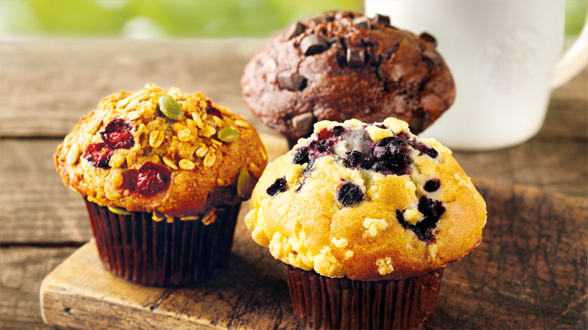
\includegraphics[width=.7\textwidth]{img/muffins.jpg} \\
     ``How many muffins of each kind?''
     \end{center}
     \end{minipage} 
       & 
     \begin{minipage}[t]{.5\textwidth}     
     \begin{center}
     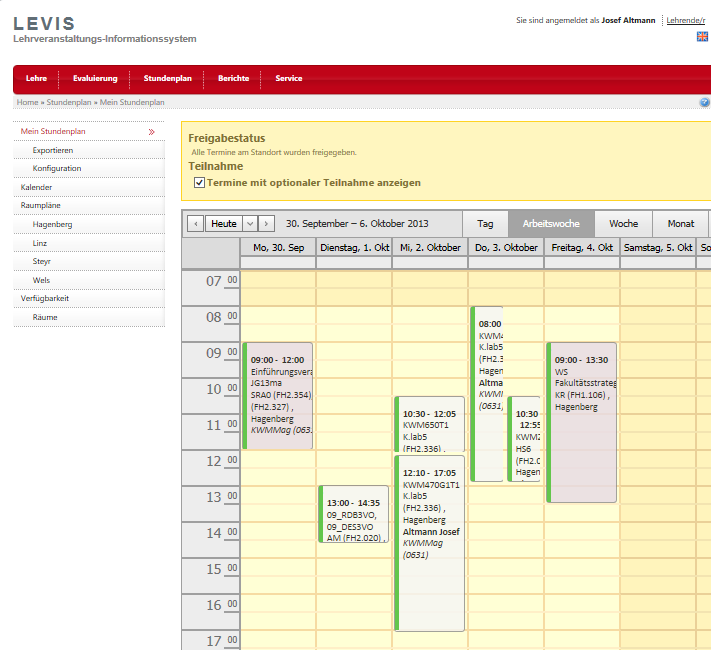
\includegraphics[width=.45\textwidth]{img/levis.png} \\
     ``When does which lecture take place?''     
       \end{center}
     \end{minipage}  \\
     \begin{minipage}[t]{.45\textwidth}     
     \begin{center}
     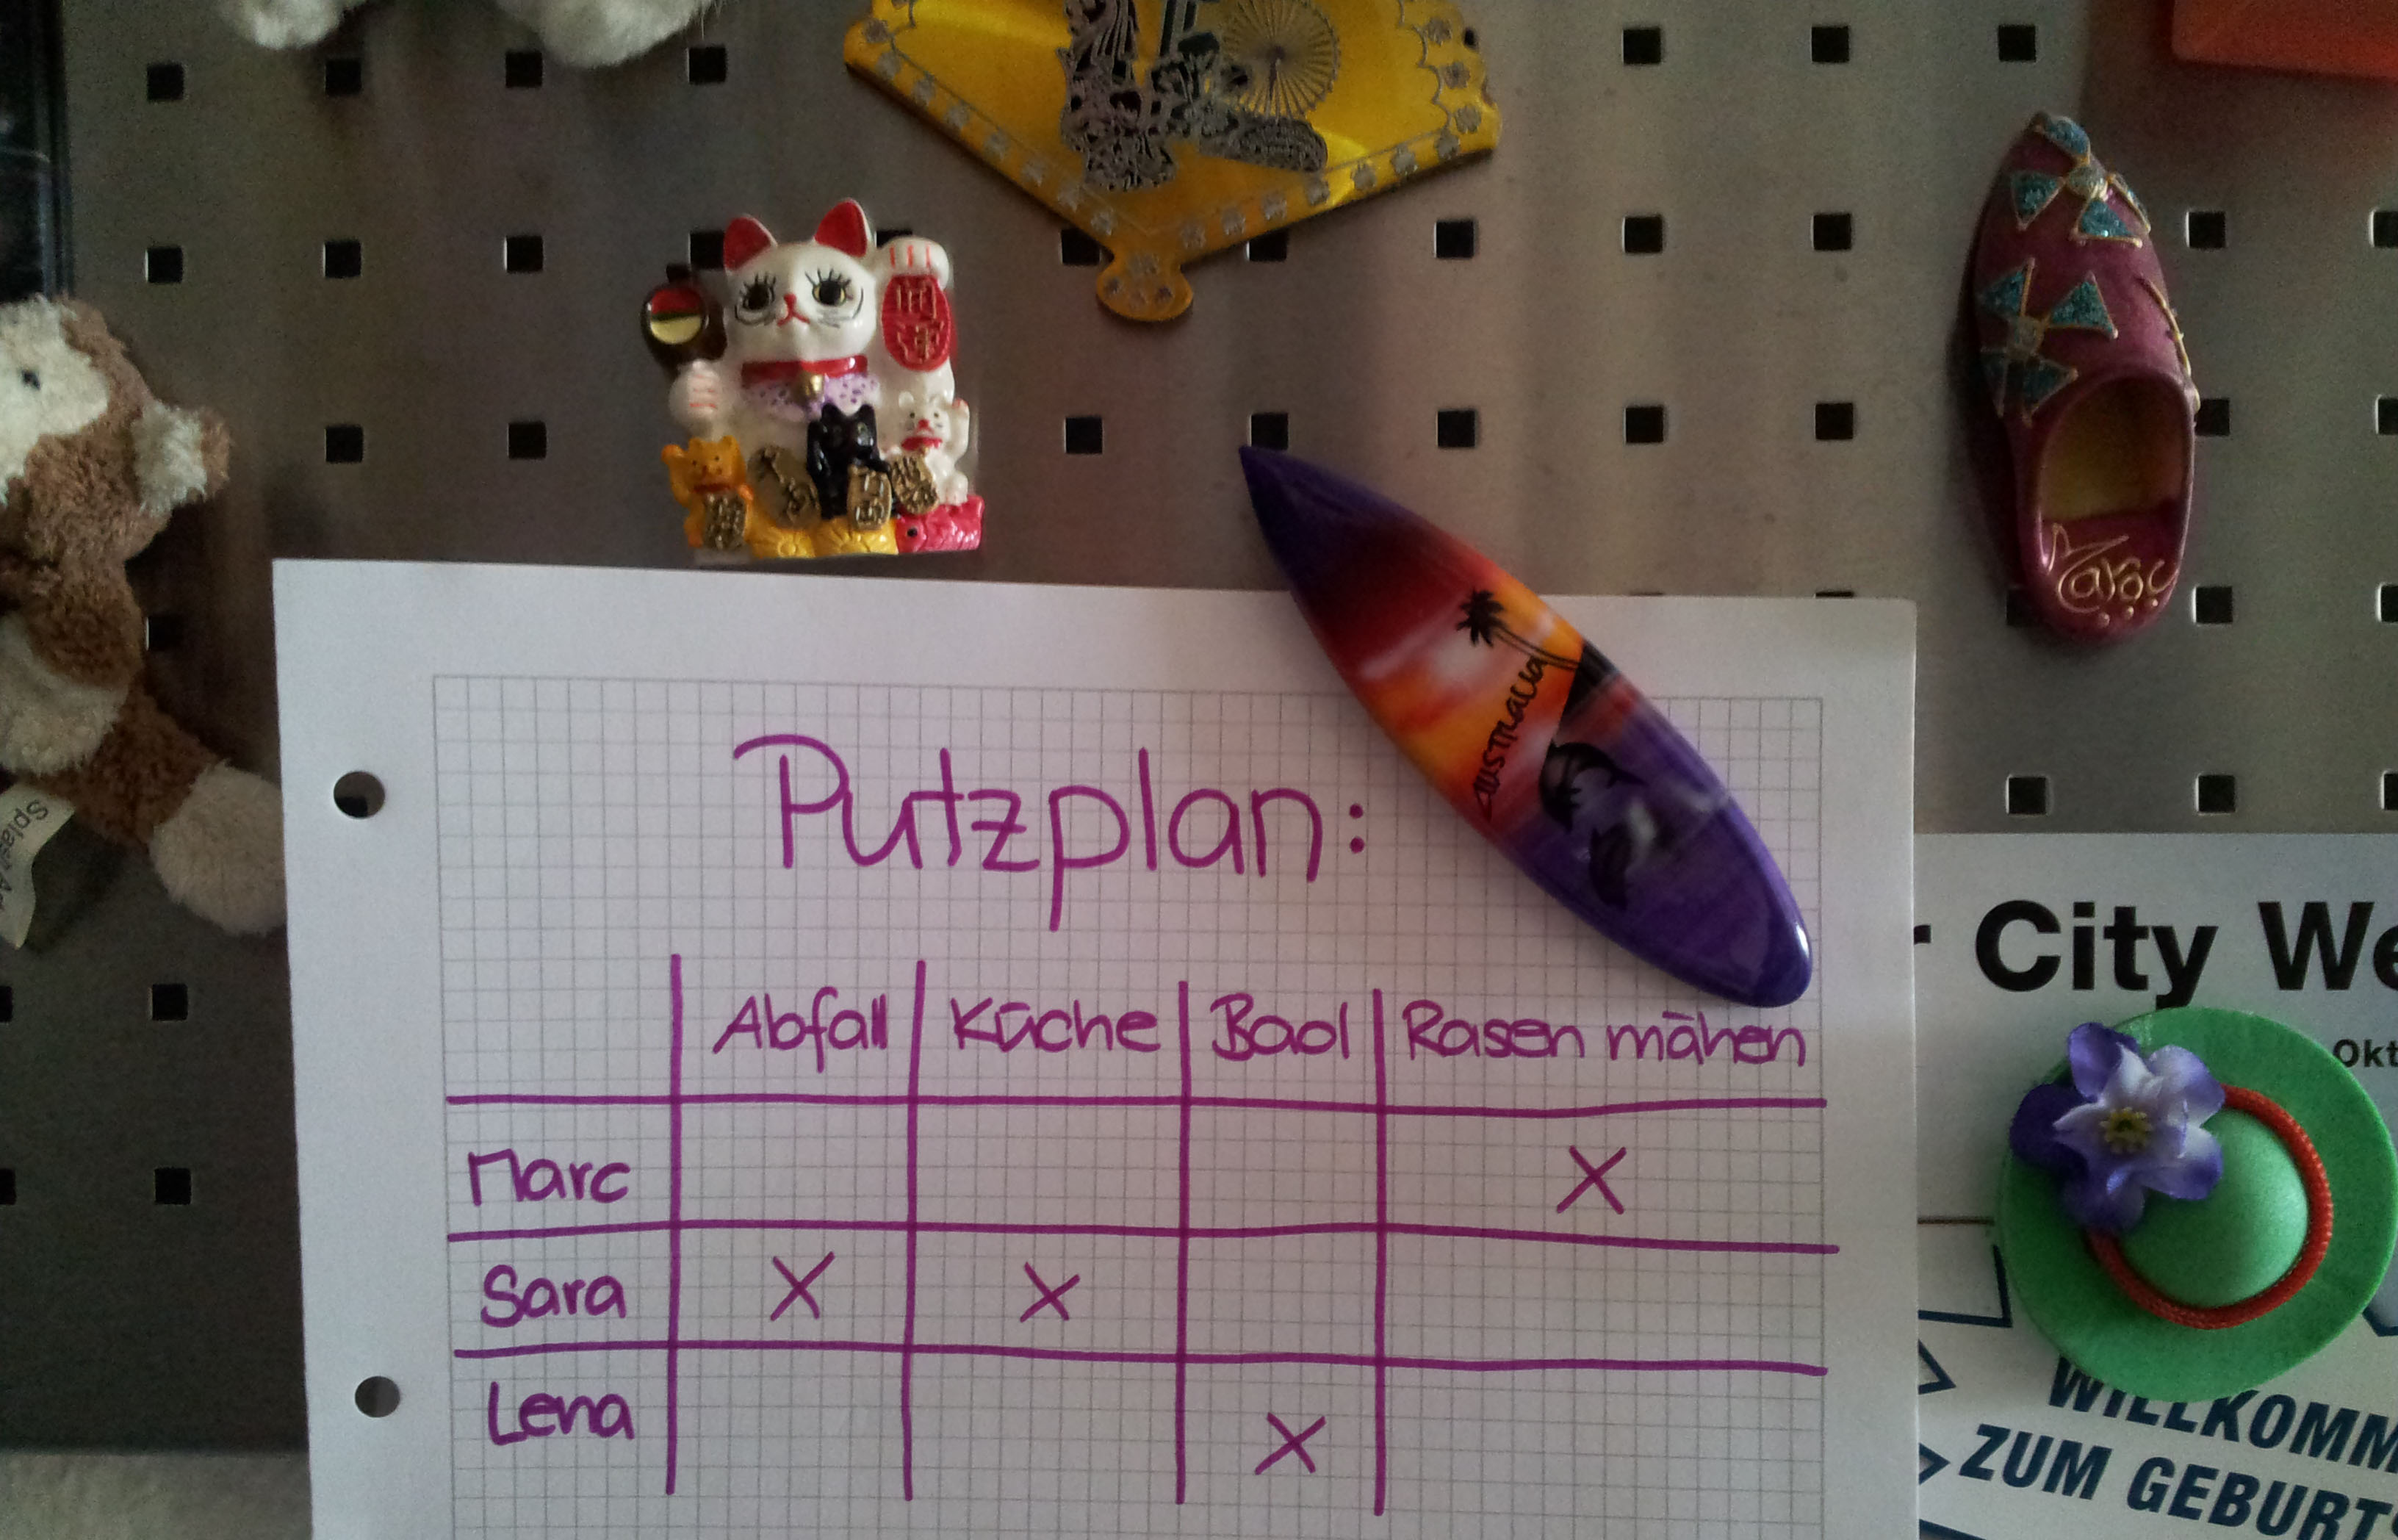
\includegraphics[width=.7\textwidth]{img/putzplan.jpg} \\
     ``Who performs which tasks?''
       \end{center}
     \end{minipage}  & 
     
     \begin{minipage}[t]{.45\textwidth}
     \begin{center}
           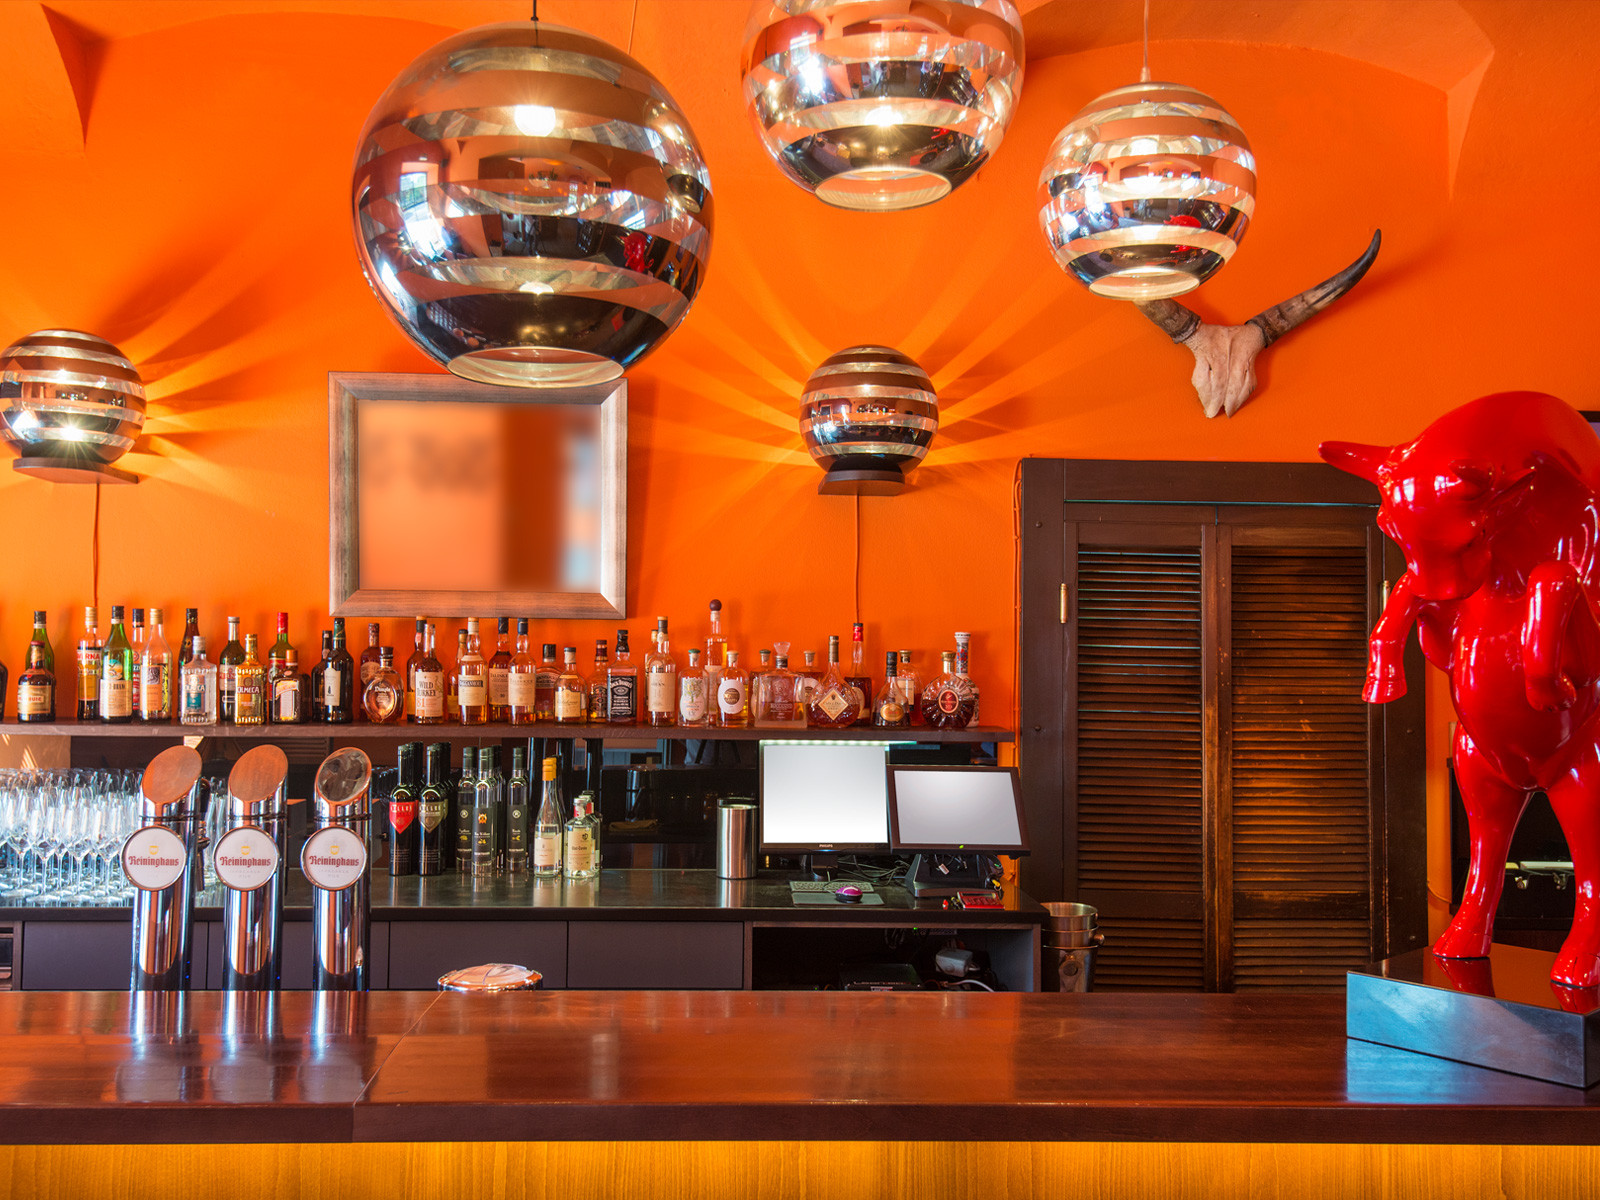
\includegraphics[width=.7\textwidth]{img/resti.jpg} \\
           ``What's up on the weekend?'' 
       \end{center}
     \end{minipage}
\\};
     
%  \path[-stealth]
%    (m-1-1) edge node [left] {$\mathcal{B}_X$} (m-2-1)
%            edge [double] node [below] {$\mathcal{B}_t$} (m-1-2)
%    (m-2-1.east|-m-2-2) edge node [below] {$\mathcal{B}_T$}
%            node [above] {$\exists$} (m-2-2)
%    (m-1-2) edge node [right] {$\mathcal{B}_T$} (m-2-2)
%            edge [dashed,-] (m-2-1);
\end{tikzpicture}

\end{center}
\end{frame}

\begin{frame}{What do these problems have in common?}
\hFirst{Decisions} \onslide<2->{\emph{(variables)}}
\begin{itemize}
\item The number of chocolate or banana muffins
\item The lectures in the curriculum
\item Friday and saturday activity
\end{itemize}
\pause

\vspace*{2ex}

\hFirst{Possibilities} \onslide<3->{\emph{(domains)}}
\begin{itemize}
\item Chocolate muffins: $\{0, \ldots, 20\}$
\item Lecture ``Algorithms 101'': $\{\mathrm{LH1}, \mathrm{LH2}, \mathrm{LH3}, \ldots \}$
\end{itemize}

\pause

\vspace*{2ex}

\hFirst{Dependencies} \onslide<4->{\emph{(constraints)}}
\begin{itemize}
\item The required flour for $x$ chocolate and $y$ banana muffins may not exceed 250g.
\item There can only be one class per room (at a time).
\item There can only be one all-you-can-eat buffet per weekend.
\end{itemize} \pause 
\end{frame}

\begin{frame}{What do these problems have in common?}
\hFirst{Preferences} \onslide<2->{\emph{(soft constraints)}}
\begin{itemize}
\item There \emph{should} be no algorithm lab on Friday, 8am
\item Bernd would like to have steaks, Ada prefers sushi $\rightarrow$ Ada's preference is \emph{more important}
\item I'd rather not clean nor vacuum. But if I have to do either, cleaning is \emph{worse}
\end{itemize}
\pause

\vspace*{2ex}
and/or
\vspace*{2ex}

\hFirst{Goals} \onslide<3->{\emph{(utility functions)}}
\begin{itemize}
\item Maximize the revenue of our chocolate/banana mix
\item Maximize the number of lecture-free days 
\end{itemize}

\vspace*{2ex}
\hfill a \alert{constraint satisfaction (optimization) problem} (CSP/COP), 

\hfill discrete if some decisions are over integers 
\end{frame}


\begin{frame}{Discrete Optimization Problems in FAS* (1)}

\begin{center}
Adaptive production cells

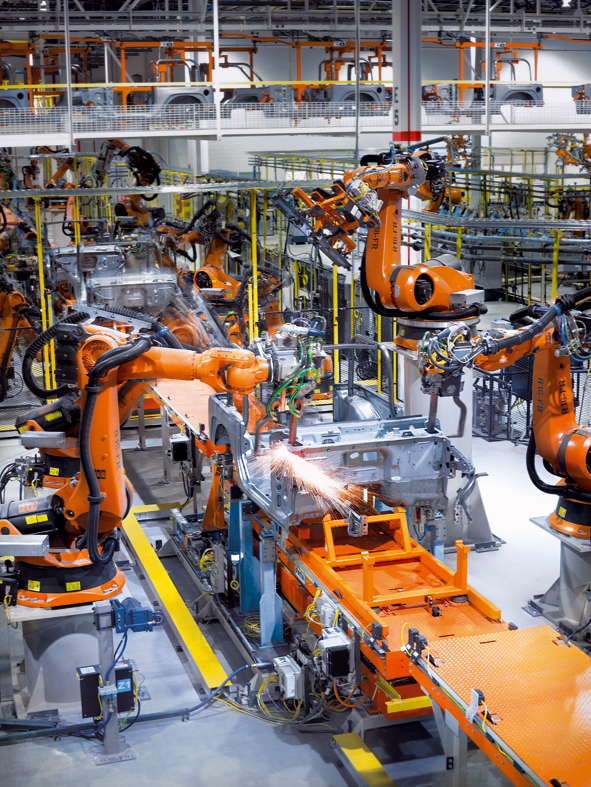
\includegraphics[width=.42\textwidth]{img/automobilindustrie.jpg}
\end{center}
\end{frame}

\begin{frame}{Discrete Optimization Problems in FAS* (1)}
\textbf{Goal}: Assign tasks to robots such that a correct \alert{resource flow} emerges
\begin{center}
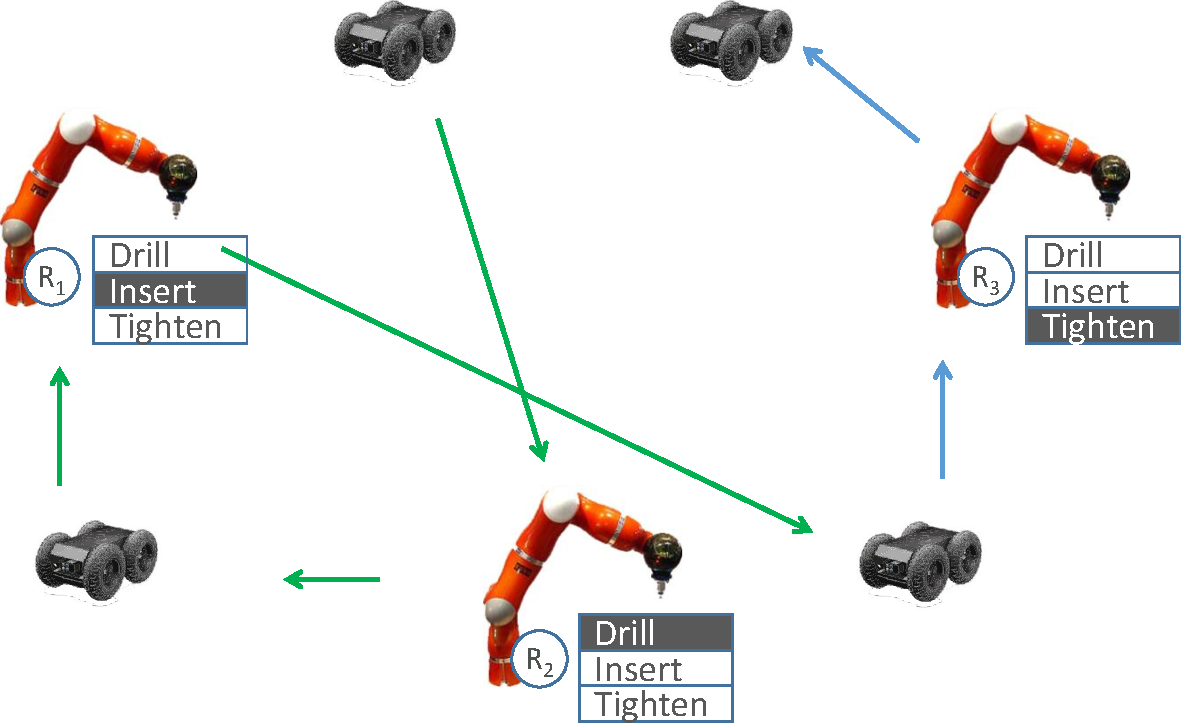
\includegraphics[width=.7\textwidth]{img/produktionszelle.pdf}
\end{center}

\hfill \cite{seebach2010software}, SASO

\end{frame}


\begin{frame}{Discrete Optimization Problems in FAS* (2)}
\begin{center}
Decentralized energy management
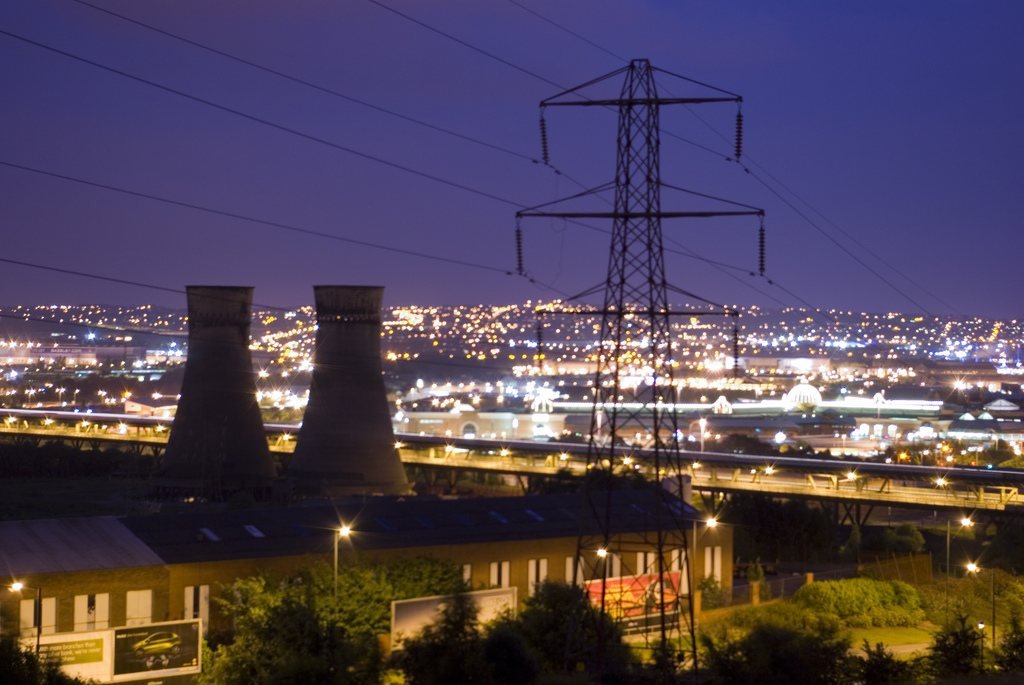
\includegraphics[width=.7\textwidth]{img/power_plants.jpg}
\end{center}
\end{frame}

\begin{frame}[fragile]{Discrete Optimization Problems in FAS* (2)}
\textbf{Goal}: Schedule power plants such that they meet the demand 
\tikzset{
    trajectory/.style={issegrey},
    emph/.style={isseorange},
    trajectorynode/.style={issegrey},
    demand/.style={MidnightBlue, thick},
    firstTraj/.style={ForestGreen},
    secTraj/.style={BrickRed}
} 
\begin{figure}
\begin{tikzpicture}[scale=1.0]
    % Draw axes
    \draw [<->,thick] (0,5) node (yaxis) [above] {$P(t)$}
        |- (8.5,0) node (xaxis) [right] {$t$};
        
    \node[overlay,text width=1.9cm, text centered, anchor=south, right] at (7.7,4.5)
    { \small 
    \begin{itemize} 
    \item[] { \color{MidnightBlue} \onslide<2->{\textbf{Demand}} } 
    \item[] { \color{ForestGreen} \onslide<3->{Plant $a$} } 
    \item[] { \color{BrickRed} \onslide<4->{Plant $b$} }  
    \item[] { \color{isseorange} \onslide<5->{\textbf{Supply}} }    
    \end{itemize}
    };        
       
	
%	\node[text width = 1.5cm ,text centered, anchor=west, right] at (2.5, 1)
%	{
%		$\mathbf{+}$
%	};
	
    %\node[text width=2.5cm, text centered, anchor=west, right] at (4,-.5)
    %{
    %		Kraftwerk $\mathsf{b}$
	%}; 
	
	%\node[text width = 1.5cm ,text centered, anchor=west, right] at (6.5, 1)
	%{
	%	$\mathbf{=}$
%	};
	%\node[text width=2.5cm, text centered, anchor=west, right] at (8,-.5)
    %{
    %		Demand
	%};      
    
     % draw second trajectory first graph 
     \onslide<2->{
    \draw[trajectory,demand] (0,3.9) coordinate (d20) -- (1,4.6) coordinate (d21);
    \draw[trajectory,demand] (d21) -- (2,4.4) coordinate (d22);
    \draw[trajectory,demand] (d22) -- (3,4.7) coordinate (d23);
    \draw[trajectory,demand] (d23) -- (4,3.5) coordinate (d24);
    \draw[trajectory,demand] (d24) -- (5,3.5) coordinate (d25);
    \draw[trajectory,demand] (d25) -- (6,3.5) coordinate (d26);
    \draw[trajectory,demand] (d26) -- (7,4.0) coordinate (d27);
    \draw[trajectory,demand] (d27) -- (8,4.5) coordinate (d28);
    
    % now for the circles
    \fill[trajectorynode,demand] (d21) circle (1pt);
    \fill[trajectorynode,demand] (d22) circle (1pt);
    \fill[trajectorynode,demand] (d23) circle (1pt);
    \fill[trajectorynode,demand] (d24) circle (1pt);    
    \fill[trajectorynode,demand] (d25) circle (1pt);
    \fill[trajectorynode,demand] (d26) circle (1pt);
    \fill[trajectorynode,demand] (d27) circle (1pt);
    \fill[trajectorynode,demand] (d28) circle (1pt);
    }
        
    \onslide<3->{
    % now for the first plant   
    \draw[trajectory,firstTraj] (0,1.9) coordinate (p10) -- (1,2.0) coordinate (p11);
    \draw[trajectory,firstTraj] (p11) -- (2,2.4) coordinate (p12);
    \draw[trajectory,firstTraj] (p12) -- (3,2.4) coordinate (p13);
    \draw[trajectory,firstTraj] (p13) -- (4,2.2) coordinate (p14);
    \draw[trajectory,firstTraj] (p14) -- (5,2.4) coordinate (p15);
    \draw[trajectory,firstTraj] (p15) -- (6,2.4) coordinate (p16);
    \draw[trajectory,firstTraj] (p16) -- (7,2.4) coordinate (p17);                   
    \draw[trajectory,firstTraj] (p17) -- (8,2.6) coordinate (p18);
    
    	\onslide<6>{
       \draw[trajectory,firstTraj,very thick] (p11) -- (p12);	
       \node[overlay,align=left,rectangle callout,%
             callout absolute pointer=(p11.west),xshift=-.5cm,yshift=-1.5cm,fill=isseorange!50] at (p12) {
            \scriptsize \textbf{Must} ramp up \\ \scriptsize due to inertia};
       
	}    
    
 	\onslide<8>{
       \draw[trajectory,firstTraj,very thick] (p15) -- (p16);	
       \draw[trajectory,firstTraj,very thick] (p16) -- (p17);
       
          \node[overlay,align=left,rectangle callout,%
             callout absolute pointer=(p16.north),xshift=-.5cm,yshift=0.55cm,fill=isseorange!50] at (p15) {
           \scriptsize  Wait 2 steps for \\ \scriptsize further ramp-up};
	} 
	
    % now for the circles of the first graph
    \fill[trajectorynode,firstTraj] (p11) circle (1pt);
    \fill[trajectorynode,firstTraj] (p12) circle (1pt);
    \fill[trajectorynode,firstTraj] (p13) circle (1pt);
    \fill[trajectorynode,firstTraj] (p14) circle (1pt);    
    \fill[trajectorynode,firstTraj] (p15) circle (1pt);
    \fill[trajectorynode,firstTraj] (p16) circle (1pt);
    \fill[trajectorynode,firstTraj] (p17) circle (1pt);
    \fill[trajectorynode,firstTraj] (p18) circle (1pt);        
    }
    
    \onslide<4->{
    % now for the second plant   
    \draw[trajectory,secTraj] (0,2.0) coordinate (p20) -- (1,2.6) coordinate (p21);
    \draw[trajectory,secTraj] (p21) -- (2,2.0) coordinate (p22);
    \draw[trajectory,secTraj] (p22) -- (3,2.2) coordinate (p23);
    \draw[trajectory,secTraj] (p23) -- (4,1.5) coordinate (p24);
    \draw[trajectory,secTraj] (p24) -- (5,1.4) coordinate (p25);
    \draw[trajectory,secTraj] (p25) -- (6,1.2) coordinate (p26);
    \draw[trajectory,secTraj] (p26) -- (7,1.6) coordinate (p27);                   
    \draw[trajectory,secTraj] (p27) -- (8,1.9) coordinate (p28);
	\onslide<6>{
       \draw[trajectory,secTraj,very thick] (p21) -- (p22);	
       \node[overlay,align=left,rectangle callout,%
             callout absolute pointer=(p21.north),xshift=+1cm,yshift=.5cm,fill=isseorange!50] at (p21) {
            \scriptsize Has to compensate};
	}    
	
	\onslide<7>{
       \draw[trajectory,secTraj,very thick] (p23) -- (p24);	
       \node[overlay,align=left,rectangle callout,%
             callout absolute pointer=(p24.south),xshift=+1cm,yshift=-.8cm,fill=isseorange!50] at (p24) {
             \scriptsize Cannot ramp down further};
	}    
    
     % now for the circles of the second graph
    \fill[trajectorynode,secTraj] (p21) circle (1pt);
    \fill[trajectorynode,secTraj] (p22) circle (1pt);
    \fill[trajectorynode,secTraj] (p23) circle (1pt);
    \fill[trajectorynode,secTraj] (p24) circle (1pt);    
    \fill[trajectorynode,secTraj] (p25) circle (1pt);
    \fill[trajectorynode,secTraj] (p26) circle (1pt);
    \fill[trajectorynode,secTraj] (p27) circle (1pt);
    \fill[trajectorynode,secTraj] (p28) circle (1pt);
    }
    
    \onslide<5->{
    % draw joint production first graph 
    \draw[trajectory,emph] (0,3.9) coordinate (s20) -- (1,4.6) coordinate (s21);
    \draw[trajectory,emph] (s21) -- (2,4.4) coordinate (s22);
    \draw[trajectory,emph] (s22) -- (3,4.6) coordinate (s23);
    \draw[trajectory,emph] (s23) -- (4,3.7) coordinate (s24);
    \draw[trajectory,emph] (s24) -- (5,3.8) coordinate (s25);
    \draw[trajectory,emph] (s25) -- (6,3.6) coordinate (s26);
    \draw[trajectory,emph] (s26) -- (7,4.0) coordinate (s27);
    \draw[trajectory,emph] (s27) -- (8,4.5) coordinate (s28);
    
	% now for the circles of the sum
    \fill[trajectorynode,emph] (s21) circle (1pt);
    \fill[trajectorynode,emph] (s22) circle (1pt);
    \fill[trajectorynode,emph] (s23) circle (1pt);
    \fill[trajectorynode,emph] (s24) circle (1pt);    
    \fill[trajectorynode,emph] (s25) circle (1pt);
    \fill[trajectorynode,emph] (s26) circle (1pt);
    \fill[trajectorynode,emph] (s27) circle (1pt);
    \fill[trajectorynode,emph] (s28) circle (1pt);
    }
    
	\node[text centered, anchor=north] at (1,0) { 1 }; \draw[thick] (1,0.05) -- (1,-.05);
	\node[text centered, anchor=north] at (2,0) { 2 }; \draw[thick] (2,0.05) -- (2,-.05);
	\node[text centered, anchor=north] at (3,0) { 3 }; \draw[thick] (3,0.05) -- (3,-.05);	
	\node[text centered, anchor=north] at (4,0) { 4 }; \draw[thick] (4,0.05) -- (4,-.05);
	\node[text centered, anchor=north] at (5,0) { 5 }; \draw[thick] (5,0.05) -- (5,-.05);
	\node[text centered, anchor=north] at (6,0) { 6 }; \draw[thick] (6,0.05) -- (6,-.05);
	\node[text centered, anchor=north] at (7,0) { 7 }; \draw[thick] (7,0.05) -- (7,-.05);	
	\node[text centered, anchor=north] at (8,0) { 8 }; \draw[thick] (8,0.05) -- (8,-.05);
	    

\end{tikzpicture}
\end{figure}  
\hfill \cite{anders2013trust}, SASO
\end{frame}



\begin{frame}{Discrete Optimization Problems in FAS*}
ESDS Deployment Problem (\emph{eventually serializable data services})

\begin{center}

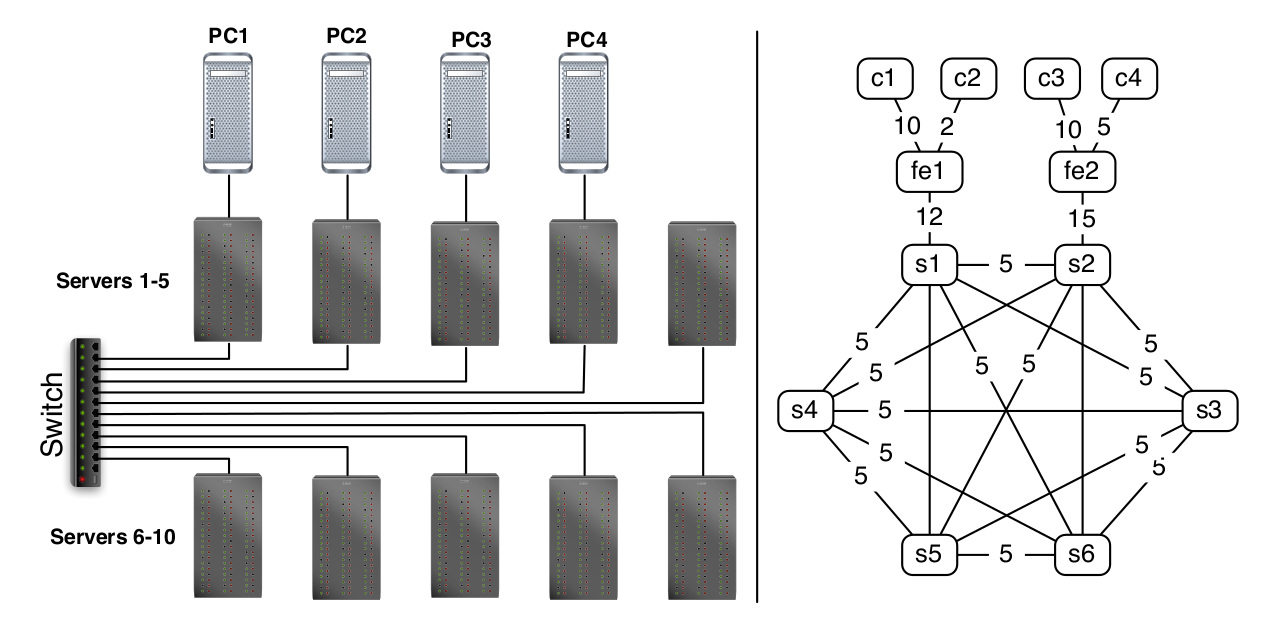
\includegraphics[width=.7\textwidth]{img/esds.png}
\end{center}
\hfill \cite{michel2008optimal}, CPAIOR
\end{frame}

\begin{frame}{Why is it useful to you?}

\alert{As a tool \ldots }

\begin{itemize}
\item If you identify discrete optimization problems in your (self-organizing, autonomic, cloud) application,
you can solve them with reliable tools.
\item Modeling languages provide \emph{easy} access to powerful solvers
\item $\rightarrow$ \emph{independent} of the concrete technology (SAT, CSP, Mathematical Programming)
\end{itemize}

\vspace*{2ex} \pause 
\alert{As a research opportunity \ldots }
\begin{itemize}
\item Studying interactions of complex networks of optimizing agents offers interesting problems (\emph{global systems science})
\item Integration of optimization problems into architectures for decision-making
\item Solving large-scale problems by decomposition through self-organization
\end{itemize}
\end{frame}



\begin{frame}
    \frametitle{Soft Constraint Programming in MiniBrass}
 \alert{Constraint programming} (first half of the tutorial)
    \begin{itemize}
    \item Declarative programming (similar to SQL, Prolog)
    \item Separation of \textbf{model} and \emph{algorithm}
    \item Suitable for combinatorial problems with hard constraints (e.g. physics!)
    \item Modeling language \hFirst{MiniZinc}
    \end{itemize}

    \vspace*{3ex}
    
\alert{Soft constraint programming} (second half of the tutorial)
    \begin{itemize} 
    \item Modeling of \textbf{user preferences}
    \item Find solutions that are \emph{as good as possible} 
    \item What does ``good`` mean?
    \item Modeling language \hFirst{MiniBrass}
     \end{itemize}
\end{frame}

\begin{frame}{Artificial Intelligence: Categories}
\begin{columns}[onlytextwidth,T]
    
    \begin{column}{.5\textwidth}
          
    \hSecond{Data-driven AI}
    \begin{center}
    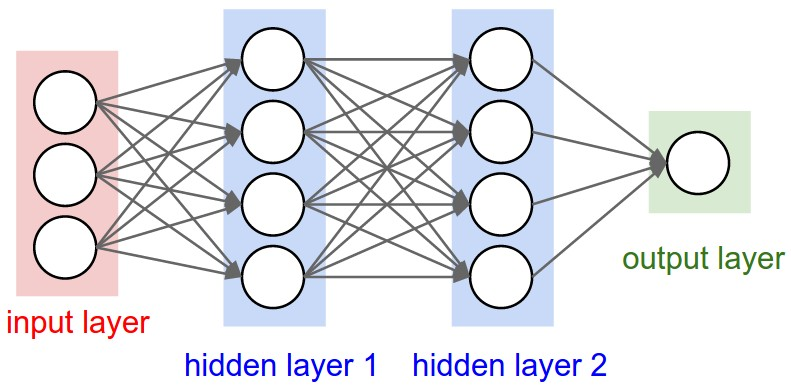
\includegraphics[width=.8\textwidth]{img/neuralnet.jpg}
    \end{center}

    \vspace*{4ex}
    
    \begin{itemize}
    \item Machine Learning
    \item Signal Processing
    \item Computer Vision
    \end{itemize}

    \end{column}
    
    \begin{column}{.5\textwidth}
    \hFirst{Decision-driven AI}
    \begin{center}
    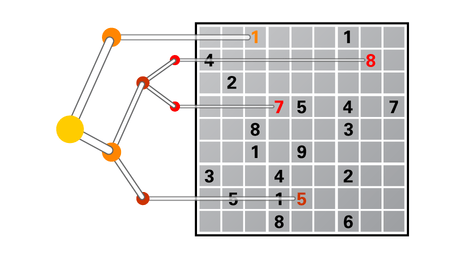
\includegraphics[width=.9\textwidth]{img/discreteopt.png}
    \end{center}
    \begin{itemize}
    \item Constraint Programming
    \item Combinatorial Optimization
    \item Heuristic Optimization
    \item Planning / Scheduling
    \end{itemize}
    
    \end{column}
  \end{columns}
\end{frame}
%


\begin{frame}[fragile]{Our first model}
\begin{lstlisting}
var 0..2: x;
var 0..2: y; 

constraint x < y;

solve maximize x + y;
\end{lstlisting}

\vspace*{2ex}

\url{http://www.minizinc.org}

\vspace*{2ex}

\small
\begin{verbatim}
x = 1;
y = 2;
----------
==========
\end{verbatim}

\end{frame}

\begin{frame}[fragile]{A second example}
\begin{lstlisting}
var 0..2: x; % this notation is shorthand for the set {0,1,2}
var 0..2: y;
var 0..1: z; % {0,1}

% c1
constraint x != y /\ y != z /\ x != z;
% c2
constraint x + 1 = y;

solve satisfy;
\end{lstlisting}
  \vspace*{3ex}
    \alert{Can you give a solution to this problem?} \pause 

\begin{itemize}
\item $\Theta = \{ (x \to 1, y \to 2, z \to \textbf{?}), (x \to 0, y \to 1, z \to \textbf{?}) \}$ satisfy $c_2$; \pause
\item $(x \to 0, y \to 1, z \to ?)$ cannot be extended to a solution since $z$ has to be 0 or 1 $\rightarrow$ has to violate 
$c_1$ \pause
\item Hence, the only solution is $(x \to 1, y \to 2, z \to 0)$
\end{itemize}
\end{frame}

\begin{frame}{Why modeling?}
\begin{enumerate}
\item Once stated (formally) -- solved many times
\begin{itemize}
\item Constraint-Solving
\item SAT -- Boolean Satisfiability
\item MIP -- Mixed Integer Programming
\item Heuristic Optimization -- Genetic etc. 
\end{itemize}
\vspace*{1ex}
\item Efficient and reliable algorithms provided by solvers
\begin{itemize}
\item Same algorithms for a variety of different problems
\item Dedicated algorithms for recurring combinatorial substructures (\texttt{alldifferent})
\end{itemize}
\vspace*{1ex}
\item Prototyping
\begin{itemize}
\item Specification becomes much clearer 
\item Bespoke algorithm for concrete problem can be developed later 
\end{itemize}

\end{enumerate}
\end{frame}

\begin{frame}[fragile]{Modeling in other CS domains}
\begin{lstlisting}[language=sql]
SELECT firstname, lastname
FROM employees 
WHERE age < 30
\end{lstlisting}
\vspace*{1ex}
instead of 
\vspace*{1ex}
\begin{lstlisting}[language=java]
Collection<Person> youngs = new ArrayList<>();
for(Person p : allEmployees) {
  if(p.getAge() < 30)
    youngs.add(p);
}
\end{lstlisting}

\begin{parchment}[Motivation]
\centering 
\alert{Constraint modeling for optimization problems $\approx$ SQL for database access} 
\end{parchment}

\end{frame}

\begin{frame}{NP-Completeness}
\begin{theorem}
The decision problem associated to a constraint satisfaction/optimization problem is NP-complete.
\end{theorem}

\begin{center}
\begin{figure}
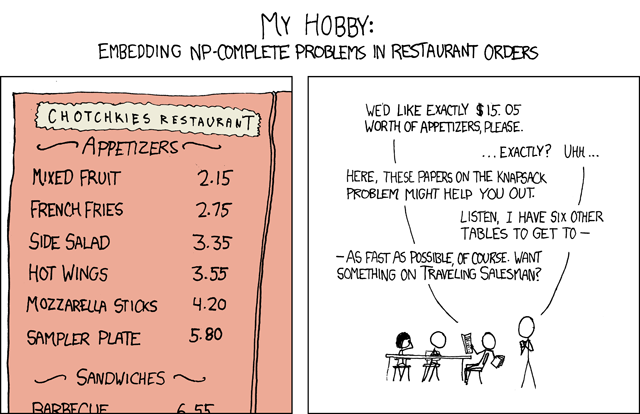
\includegraphics[width=.7\textwidth]{img/np_complete.png}
\caption{\url{https://xkcd.com/287/} }
\end{figure}
\end{center}
\end{frame}

\begin{frame}{Why MiniZinc?}
\begin{parchment}[Rationale]
\centering 
\alert{One modeling language -- many solvers} 
\end{parchment}
\begin{textblock*}{2.cm}[1,1](\textwidth-.5cm,\textheight-1.03cm)


\includegraphics[width=\textwidth]{img/MiniZn_logo.jpg} 

\end{textblock*}
Supported solvers (selection)
\begin{itemize}
\item Gecode (CP)
\item JaCoP (CP)
\item Google Optimization Tools (CP)
\item Choco (CP)
\item G12 (CP/LP/MIP)
\end{itemize}

\end{frame}

\begin{frame}[fragile]{A relevant example \ldots}
\small
\lstinputlisting{models/cakes.mzn}
\end{frame}
\begin{frame}[fragile]{Basic MiniZinc: Parameters and Variables}
\textbf{Parameters}: input data for the problem, constants 
\begin{lstlisting}
int: n; 
n = 3; 
% equivalent to: 
int: n = 3; 
par int: n = 3; 
% or with bounded domains
0..10: m; % a fixed value (input by a user) between 0 and 10
% set types 
set of int: AGENTS = 1..n; % {1, ..., n}
\end{lstlisting}
\pause 

\vspace*{2ex}

\textbf{Decision Variables}: variables to be assigned by a solver
\begin{lstlisting}
var int: n; 
var 0..10: x;
% immediate declaration (useful for dependent expressions)
var int: y = 2*x; 
\end{lstlisting}
\end{frame}

\begin{frame}[fragile]{Basic MiniZinc: Arrays and Sets}
\textbf{Arrays}: for parameters/variables of different sizes 
\begin{lstlisting}
int: n;
array[1..n] of int: height; % height[i] denotes the height of truck i
% also for decisions 
array[1..n] of var bool: x; % x[i] holds if we select item i 
% typical usage 
set of int: ITEMS = 1..n;
array[ITEMS] of var bool: x;
\end{lstlisting}
\pause 

\vspace*{2ex}

\textbf{Sets}: set type for parameters and decisions (only set of int/subtype int)
\begin{lstlisting}
set of int: AGENTS = 1..n;
set of int: CAP = 1..m; 
array[AGENTS] of set of CAP: offers; % [{1}, {2], {1,2}]

var set of AGENT: selectedTeam;
\end{lstlisting}
\end{frame}

\begin{frame}[fragile]{Basic MiniZinc: Types}
Allowed primitive types for variables/parameters are
\begin{itemize}
\item Integer \texttt{int} or subtypes:
\begin{itemize}
\item range \texttt{1..n}
\item explicit set \texttt{\{1,5,7\}}
\end{itemize}  
\item Floating point number \texttt{float} or subtypes:
\begin{itemize}
\item range \texttt{0.0 .. 1.0}
\item explicit set \texttt{\{1.0, 2.5, 3.7\}}
\end{itemize}
\item Boolean \texttt{bool}  
\item Arrays, Sets
\end{itemize}
\end{frame}

\begin{frame}[fragile]{Constraints, Objective and Output}
\textbf{Constraints}: to restrict assignments 
\begin{lstlisting}
var 0..10: x; var 0..10: y; var 0..10: z;
constraint x + y = z;
constraint x mod 2 = 0;
% 'forall' concept for arrays
par int: n; array[1..n] of var 0..10: t; 
% each t[i] should be even:
constraint forall(i in 1..n) (t[i] mod 2 = 0);
\end{lstlisting}
\pause 

\vspace*{1ex}

\textbf{Solve Item}: provides the objective (one per model)
\begin{lstlisting}
solve satisfy; % for a satisfaction problem
solve maximize sum(i in 1..n) (t[i]);
solve minimize x + y;
\end{lstlisting}
\pause 
\vspace*{1ex}

\textbf{String Output}: one output item per model
\begin{lstlisting}
var 0..10: x;
output ["The value of x is: \(x)"]
\end{lstlisting}
\end{frame}

\begin{frame}{MiniZinc: HelloWorld}
\textbf{Exercise 1}

Build a MiniZinc model \texttt{xopt.mzn} with a decision variable $x$ taking values from 0 to 10, with
constraints to ensures that $x$ is divisible by 4, which outputs the value of $x$ that gives the minimum
value of $(x-7)^2$.

Test it using the precompiled IDE-bundle. Suppose you cannot use the \texttt{mod} function, how would you alternatively model that $x$
is divisible by 4?

\end{frame}

\begin{frame}{MiniZinc: Arrays}
\textbf{Exercise 2}
Define a MiniZinc model \texttt{array.mzn} which takes an integer parameter $n$ defining the length of an
array of numbers $x$ taking values from 0 to 9. Constrain the array so the sum of the numbers in
the array is equal to the product of the numbers in the array. Output the resulting array.
Test your model using the ``all solutions'' setting active in the IDE.

\vspace*{2ex}

 Add a constraint to ensure that the numbers in the array are non-decreasing, i.e. $x[1] \leq x[2] \leq
\ldots \leq x[n]$. This should reduce the number of similar solutions. 
How big a number can you solve with your model? Why do you think this happens?


\end{frame}


\begin{frame}{Deciding functions}
\begin{itemize}
\item A very important, recurring problem is \emph{deciding} a finite \alert{function}.
\item Given 
\begin{itemize}
\item[-] Domain \texttt{DOM}
\item[-] Codomain \texttt{COD}
\end{itemize} 
\item Find a function $f : \mathtt{DOM} \to \mathtt{COD}$ 
\item Satisfying some criteria (e.g. \emph{injectivity})
\end{itemize}
\vspace*{1ex}
\pause 
Examples:
\begin{itemize}
\item Task allocation (maps tasks to workers, exactly one worker per task)
\item Exam schedules (map students to appointments, certainly different appointments)
\end{itemize}
\end{frame}

\begin{frame}{Task allocation in practice}
\begin{itemize}
\item Task allocation problem

\begin{itemize}
\item [-] $n$ robots 
\item [-] $m$ tasks
\item [-] Assign each robot a \emph{different} task and maximize the profit
\end{itemize}
\item Example:
\begin{itemize}
\item[-] $n = 4$, $m = 5$
\end{itemize}
\end{itemize}
\centering
\begin{tabular}{|c|c|c|c|c|c|}
\hline 
 & t1 & t2 & t3 & t4 & t5 \\ 
\hline 
r1 & 7 & 1 & 3 & 4 & 6 \\ 
\hline 
r2 & 8 & 2 & 5 & 1 & 4 \\ 
\hline 
r3 & 4 & 3 & 7 & 2 & 5 \\ 
\hline 
r4 & 3 & 1 & 6 & 3 & 6 \\ 
\hline 
\end{tabular} 
\end{frame}


\begin{frame}[fragile]{Task allocation: Model}
\begin{lstlisting}
% problem data 
int: n; set of int: ROBOTS = 1..n;
int: m; set of int: TASKS = 1..m;
array[ROBOTS,TASKS] of int: profit;

% decisions
array[ROBOTS] of var TASKS: allocation;

% goal
solve maximize sum(r in ROBOTS) (profit[r, allocation[r]] );

% have robots work on different tasks
constraint forall(r1 in ROBOTS, r2 in ROBOTS where r1 < r2) 
  ( allocation[r1] != allocation[r2] );
\end{lstlisting}
\end{frame}

\begin{frame}[fragile]{Judgement}
\begin{lstlisting}
constraint forall(r1 in ROBOTS, r2 in ROBOTS where r1 < r2) 
  ( allocation[r1] != allocation[r2] );
\end{lstlisting}
\begin{itemize}
\item In principle, \emph{fine}, but \ldots
\begin{itemize}
\item[-] Not very concise -- can be messed up
\item[-] $O(n^2)$ individual constraints between two variables
\end{itemize}
\pause 

\vspace*{1ex}

\item But in fact, this substructure is so common that it deserves a \emph{name}
\begin{itemize}
\item[-] \texttt{alldifferent}
\end{itemize}
\end{itemize}
\begin{lstlisting}
constraint alldifferent(allocation);
\end{lstlisting}
\begin{itemize}
\item $\mathrm{alldifferent}([x_1, \ldots, x_n]$ is true if and only if all variables $x_1$ to $x_n$ take a different value
\item e.g. $\mathrm{alldifferent}([2,3,5])$ holds but $\mathrm{alldifferent}([2,2,3])$ does not.
\end{itemize}
\end{frame}

\begin{frame}[fragile]{Task allocation: Improved Model}
\begin{lstlisting}
% problem data 
int: n; set of int: ROBOTS = 1..n;
int: m; set of int: TASKS = 1..m;
array[ROBOTS,TASKS] of int: profit;

% decisions
array[ROBOTS] of var TASKS: allocation;

% goal
solve maximize sum(r in ROBOTS) (profit[r, allocation[r]] );

include "alldifferent.mzn"; % we have to import from the library
% have robots work on different tasks
constraint alldifferent(allocation);
\end{lstlisting}
\end{frame}

\begin{frame}[fragile]{AllDifferent -- Propagation}

\begin{lstlisting}
var {1,2,3}: x;       var {2,3}: y;      var {2,3}: z;
var {1,2,3,4,5}: t; var {3,4,5,6}: u;
constraint alldifferent([x,y,z,t,u]);
\end{lstlisting}
\vspace*{-15ex}
\begin{center}
\tikzset{onslide/.code args={<#1>#2}{%
  \only<#1>{\pgfkeysalso{#2}}
}}
\tikzstyle{highlight}=[isseorange,ultra thick]
\tikzstyle{impo}=[dashed]
\begin{tikzpicture}[every node/.style={
anchor=base,
text depth=.5ex,
text height=2ex,
minimum height=2ex,
align=center,
circle,
text width=1em}]
\matrix (magic) [nodes in empty cells, ampersand replacement=\&,row sep=0.3cm,column sep=0.5cm]
{
\node[draw, circle](x){$x$}; \& \node[draw, circle](y){$y$};  \& \node[draw, circle](z){$z$};  \& \node[draw, circle](t){$t$};  \& \node[draw, circle](u){$u$};  \\
 \& \\
\& \\
\& \\
\node[draw, circle](1){$1$};  \& \node[draw, circle](2){$2$};  \& \node[draw, circle](3){$3$};  \& \node[draw, circle](4){$4$};  \& \node[draw, circle](5){$5$};  \& \node[draw, circle](6){$6$};  \\
};

\draw[onslide={<2>{highlight}}] (x) -- (1);
\draw[onslide={<2>{impo}}] (x) -- (2);
\draw[onslide={<2>{impo}}] (x) -- (3);

\draw[onslide={<2>{highlight}}] (y) -- (3);
\draw[] (y) -- (2);

\draw[onslide={<2>{highlight}}] (z) -- (2);
\draw[] (z) -- (3);

\draw[onslide={<2>{highlight}}] (t) -- (5);
\draw[onslide={<2>{impo}}] (t) -- (1);
\draw[onslide={<2>{impo}}] (t) -- (2);
\draw[onslide={<2>{impo}}] (t) -- (3);
\draw[] (t) -- (4);
\draw[onslide={<2>{highlight}}] (u) -- (4);
\draw[onslide={<2>{impo}}] (u) -- (3);
\draw[] (u) -- (5);
\draw[] (u) -- (6);
\end{tikzpicture}
\end{center}
\vspace*{-15ex}
\begin{lstlisting}
var {1}: x;       var {2,3}: y;      var {2,3}: z;
var {4,5}: t;      var {4,5,6}: u;
constraint alldifferent([x,y,z,t,u]);
\end{lstlisting}
\end{frame}

\begin{frame}{Other Globals}
Assume an employee scheduling problem (rostering) 

(Shifts: 1 = morning, 2 = afternoon, 3 = night):

%\vspace*{2ex}
\begin{center}
\begin{tabular}{|c|c|c|c|c|c|}
\hline 
 & Monday & Tuesday & Wednesday & Thursday & Friday \\ 
\hline 
Nurse 1 & off & 1 & \alert<2->{2} & 3 & 2 \\ 
Nurse 2 & 1 & off & \alert<2->{1} & 1 & 1 \\ 
Nurse 3 & 1 & 2 & off & 1 & 2 \\ 
Nurse 4 & 2 & 2 & \alert<2->{2} & off & 3 \\ 
Nurse 5 & \alert<3->{3} & \alert<3->{3} & \alert<2->{2} & \alert<3->{3} & off \\ 
\hline 
\end{tabular} 
\end{center}
\pause 
\begin{itemize}
\item Consider work regulations
\begin{itemize} \pause 
\item At least one nurse has to be assigned to every shift per day \pause 
\item Each nurse may at most work two night shifts
\item Each nurse needs to have one day off 
\end{itemize}
\end{itemize}

\end{frame}

\begin{frame}[fragile]{Cardinality Constraint}

\begin{center}
\begin{tabular}{|c|c|c|c|c|c|}
\hline 
$\mathsf{worksShift}$ & Monday & Tuesday & Wednesday & Thursday & Friday \\ 
\hline 
Nurse 1 & off & 1 & 2 & 3 & 2 \\ 
Nurse 2 & 1 & off & 1 & 1 & 1 \\ 
%Nurse 3 & 1 & 2 & off & 1 & 2 \\ 
%Nurse 4 & 2 & 2 & 2 & off & 3 \\ 
%Nurse 5 & 3 & 3 & 2 & 3 & off \\ 
\hline 
\end{tabular} 
\end{center}%
\begin{itemize}
\item $\mathrm{cardinality}(X \mid v, l, u)$
\begin{itemize}
\item $X = \{x_1, \ldots, x_n\}$
\item $v = (v_1, \ldots, v_m)$
\item $l = (l_1, \ldots, l_m)$ contain \emph{lower} and 
$u = (u_1, \ldots, u_m)$ \emph{upper} bounds for values $v_i$ 
\end{itemize}

\vspace*{1ex} \pause

\item For instance, for each nurse $i$:
\begin{itemize}
\item[-] $\mathrm{cardinality}([ \mathsf{worksShift}[i, \cdot] ] \mid (0,1,2,3), (1,0,0,0), (5, 5, 5, 2))$
\end{itemize} 
\item In MiniZinc:
\end{itemize}
\begin{lstlisting}
constraint forall(i in NURSES) (
       global_cardinality_low_up([worksShift[i,d] | d in DAYS], 
                                 [0,1,2,3], [1,0,0,0], [1,5,5,2] ) );
\end{lstlisting}
\end{frame}
\begin{frame}{MiniZinc: Group Photo}
\textbf{Exercise 3}

Given a group of $n$ people, we must arrange them for a photo. The best
photo is when people are next to their friends, so the aim is to arrange them so that each person
is next to (to the left or right) with as many friends as possible. The data for the
problem is given as
%
\begin{align*}
& \texttt{n = <size of problem> ;} \\
& \texttt{array[1..n,1..n] of var bool: friend; }
\end{align*} 
%
where \texttt{friend[f1, f2]} means \texttt{f1} and \texttt{f2} are friends. You can assume that the friend array is symmetric.
You should output a list of the people in their position to maximize the number of adjacent
friends. For example given the data \texttt{groupphoto1.dzn}, you should output the placement of the guests as well as the objective value, i.e.,

\begin{align*}
& \texttt{Obj = 7; [4, 3, 5, 6, 8, 7, 1, 2]}
\end{align*}


\end{frame}


%
\begin{frame}{Praxis I}
Third International CSP Competition (CPAI’08)
\begin{center}
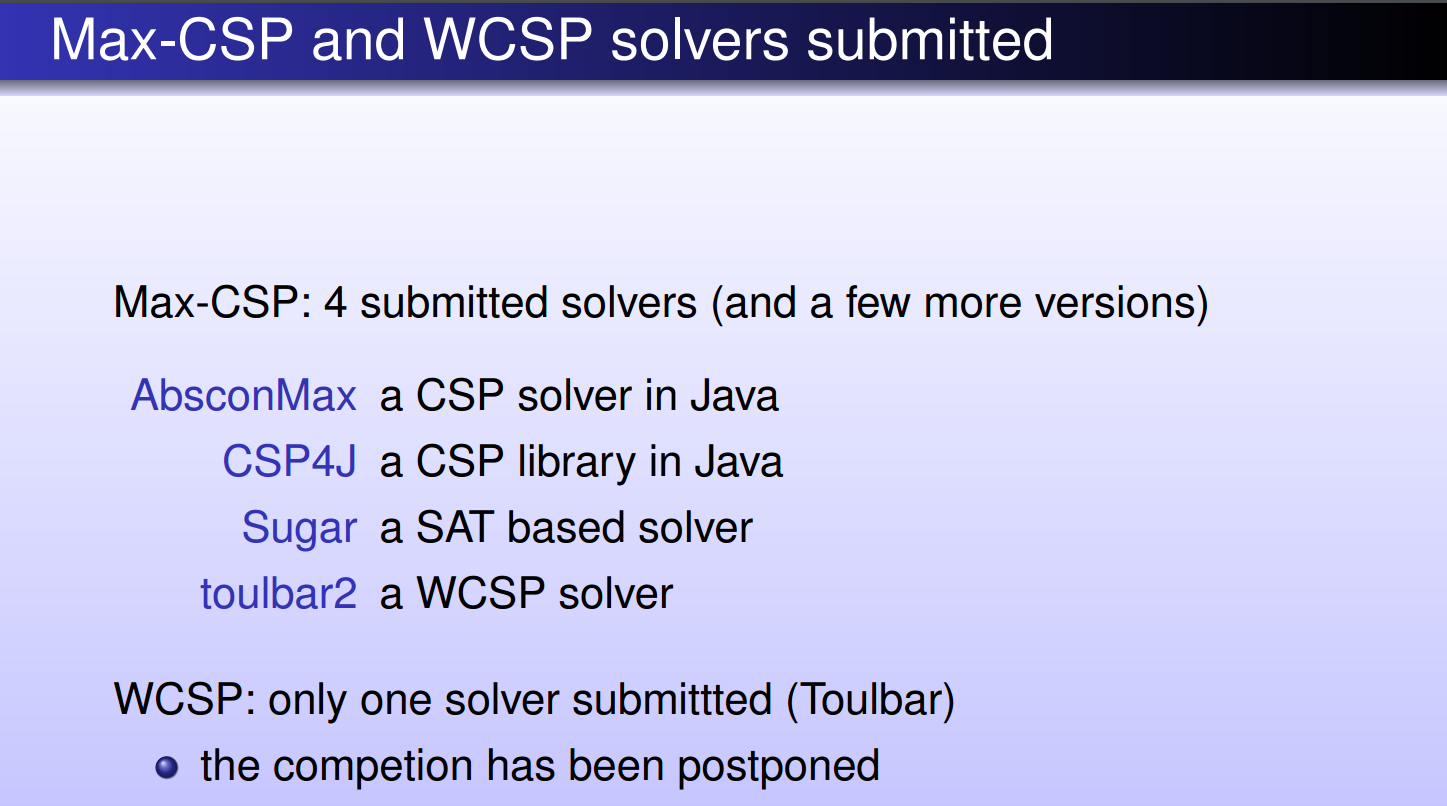
\includegraphics[width=.8\textwidth]{img/cpai08.png}
\end{center}
\end{frame}

\begin{frame}{Praxis II}
Im Constraint Programming:
\begin{itemize}
\item Fokus auf \emph{klassischen} Constraint-Lösern
\item Erweiterung auf einfache Optimierung (Branch \& Bound)
\item Zielfunktion kann skalare Variable (\texttt{int} oder \texttt{float}) sein
\item { \color{isseorange} \texttt{toulbar2} ist der einzige dedizierte Weighted-CSP-Solver}
\end{itemize}

\vspace*{2ex}

In der mathematischen Programmierung:

\begin{itemize}
\item Probleme müssen gewisse Struktur aufweisen (lineare Constraints, quadratische Constraints, etc.)
\item Schlecht geeignet für beliebige Ordnungen nach denen optimiert werden soll
\end{itemize}

\vspace*{1ex} \pause 
Wir wollen aber heterogene PVS $\rightarrow$ \alert{MiniZinc}
\end{frame}


\begin{frame}{Warum MiniZinc?}
\begin{parchment}[Rationale]
\centering 
\alert{Eine Modellierungssprache -- viele Solver} 
\end{parchment}

\begin{textblock*}{2.cm}[1,1](\textwidth-.5cm,\textheight-1.03cm)


\includegraphics[width=\textwidth]{img/MiniZn_logo.jpg} 

\end{textblock*}
\emph{Reduziere Soft-Constraint-Probleme auf konventionelle Constraint-Probleme}

\begin{itemize}
\item Gecode (CP)
\item JaCoP (CP)
\item Google Optimization Tools (CP)
\item CPLEX (CP/LP/MIP)
\item G12 (CP/LP/MIP)
\item \ldots
\end{itemize}
\end{frame}

\begin{frame}{MiniZinc: Entwicklungszustand}

\end{frame}

%
\tikzstyle{highlight}=[isseorange,ultra thick]
\begin{frame}[plain]
\begin{center}
\begin{tikzpicture}[scale=0.77,auto]

% single PVS
\node (bot) at (0,0) {\alert{$\bot = \lbag c_1, c_2, c_3 \rbag$}};
\node (c1c2) at (-2,1) {\alert<2->{$\lbag c_1, c_2 \rbag$}};
\node (c2c3) at (0,2) {$ \lbag c_2, c_3 \rbag$};
\node (c1c3) at (2,1) {$\lbag c_1, c_3 \rbag$};

\node (c1) at (0,3) {\alert<3->{$\lbag c_1 \rbag$}};
\node (c2) at (-2,4) {\alert<4->{$\lbag c_2 \rbag$}};
\node (c3) at (2,4) {$\lbag c_3 \rbag$};
%\node (a) at (-1,0.5) {$a$};
%\node (b) at (-1,1.5) {$b$};
%\node (c) at (1,1) {$c$};
\node (top) at (0,5) {$\top = \lbag \rbag $};

\node[text width=2cm] (verb) at (4,0) {     };
\path[-]
(bot) edge[highlight] (c1c2)
      edge (c2c3)
      edge (c1c3)
(c1c2) edge (c2c3)
(c1c3) edge (c2c3)
(c1c3) edge (c1)
(c1c3) edge (c3)
(c2c3) edge (c2)
(c2c3) edge (c3)
(c1c2) edge[highlight] (c1)
(c1c2) edge (c2)
(c1) edge[highlight] (c2)
(c1) edge (c3)
(c2) edge (top)
(c1) edge (top)
(c3) edge (top)
      ;
%(a) edge (b)
%(b) edge (top)
%(bot) edge (c)
%(c) edge (top)
;

\end{tikzpicture}
\end{center}
\end{frame}

\begin{frame}[plain]
\begin{center}
\begin{tikzpicture}[scale=0.77,auto]

% single PVS
\node (bot) at (0,0) {\alert{$\bot = k$}};
\node (k-1) at (0,1) {\alert{$k-1$}};
\node (k-2) at (0,2) {\alert{$k-2$}};

\node (dots) at (0,3) {$\ldots$};
\node (1) at (0,4) {$1$};
\node (top) at (0,5) {$\top = 0 $};

\node[text width=2cm] (verb) at (4,0) {     };
\path[-]
(bot) edge[highlight] (k-1)
(k-1) edge[highlight] (k-2)
(k-2) edge (dots)
(dots) edge (1)
(1) edge (top)
      ;
%(a) edge (b)
%(b) edge (top)
%(bot) edge (c)
%(c) edge (top)
;

\end{tikzpicture}
\end{center}
\end{frame}

%
\begin{frame}{Case Studies}
MiniBrass has been used in several applications:

\vspace*{2ex}

\begin{itemize}
\item \alert<2->{Student-Mentor-Matching}
\item Exam Scheduling
\item Distributed Power Systems
\item Multi-User-Multi-Display (User Preferences)
\item Reconfigurable robot teams 
\end{itemize}
\end{frame}



\begin{frame}[fragile]{Mentor Matching}

\textbf{Goal}: Assign mentees (e.g. students) to mentors (e.g. companies), such that
\begin{itemize}
\item Students are very content with their mentors
\item Companies like their mentees as well
\item Two-sided preferences
\end{itemize}

\vspace*{2ex}

Sounds like a typical \emph{stable matching}-problem, but:

\begin{itemize}
\item There is no 1:1 mapping (companies supervise several students)
\item Additional side constraints are present:
\begin{itemize}
\item[-] Each company supervises at least $l$, at most $u$ students
\item[-] The number of supervised students \emph{should} be roughly equal (Fairness)
\item[-] Students that despise one company should not be forced to work with them 
\end{itemize}
\end{itemize}
\end{frame}


\begin{frame}[fragile]{Mentor Matching: Example}
\begin{center}
\tikzset{onslide/.code args={<#1>#2}{%
  \only<#1>{\pgfkeysalso{#2}}
}}

\tikzstyle{highlight}=[isseorange,ultra thick]
\tikzstyle{highlight2}=[CornflowerBlue,ultra thick,rounded corners]
\tikzstyle{defaultStyle}=[white,ultra thick,rounded corners]

\tikzstyle{impo}=[dashed]
\begin{tikzpicture}[every node/.style={
anchor=base,
%text depth=.5ex,
%text height=2ex,
%minimum height=2ex,
align=center,
rectangle,
text width=2em
}]
\matrix (magic) [nodes in empty cells, ampersand replacement=\&,row sep=0.4cm,column sep=1.5cm]
{
\node[draw,defaultStyle, onslide={<3->{highlight2}}](s1){
\includegraphics[width=\textwidth]{img/businessman.png}}; \& \& \& \node[text width=4em, defaultStyle, draw, onslide={<3->{highlight2}}](c1) {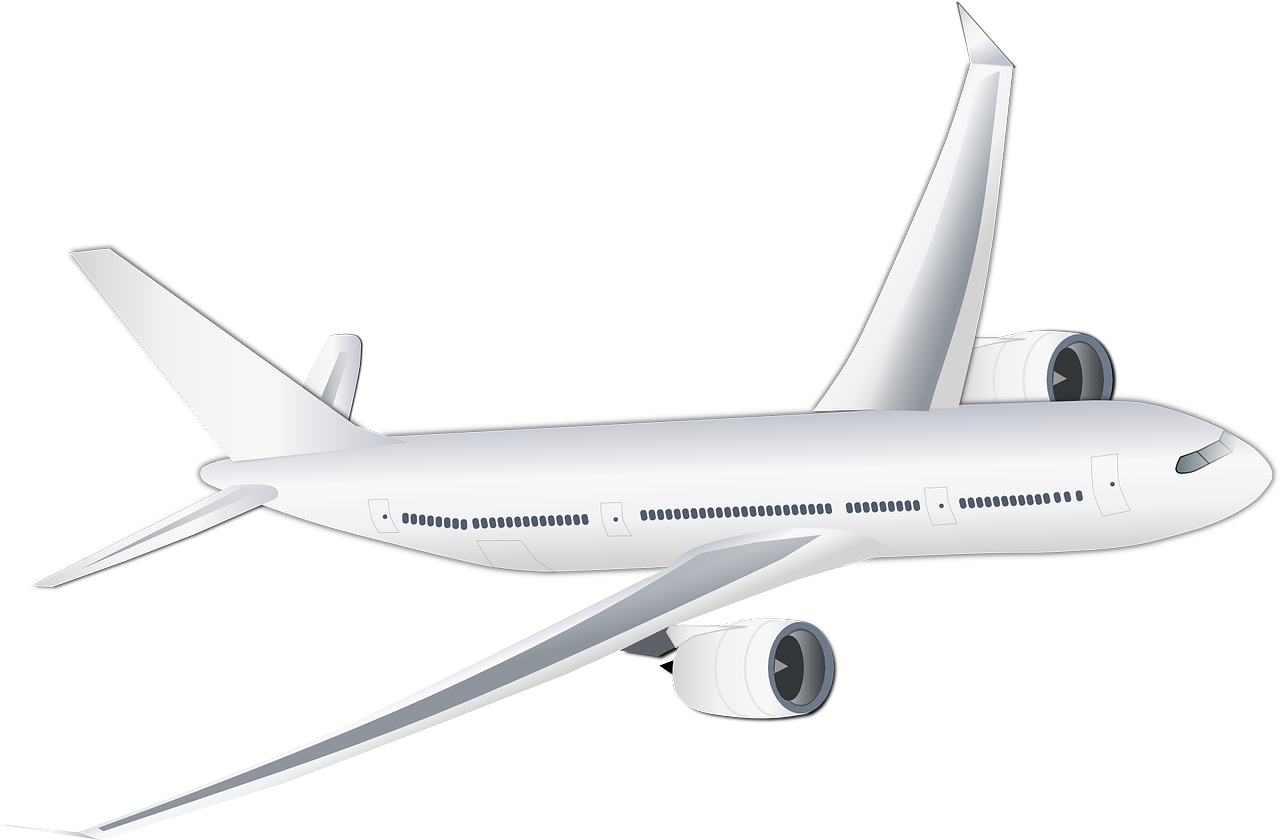
\includegraphics[width=\textwidth]{img/airplane.png}}; \\
\node(s2){
\includegraphics[width=\textwidth]{img/woman.png}};       \& \& \& \node(c2) {
\includegraphics[width=2\textwidth]{img/logistics.png}}; \\
\node(s3){
\includegraphics[width=\textwidth]{img/man.png}};         \& \& \& \node(c3) {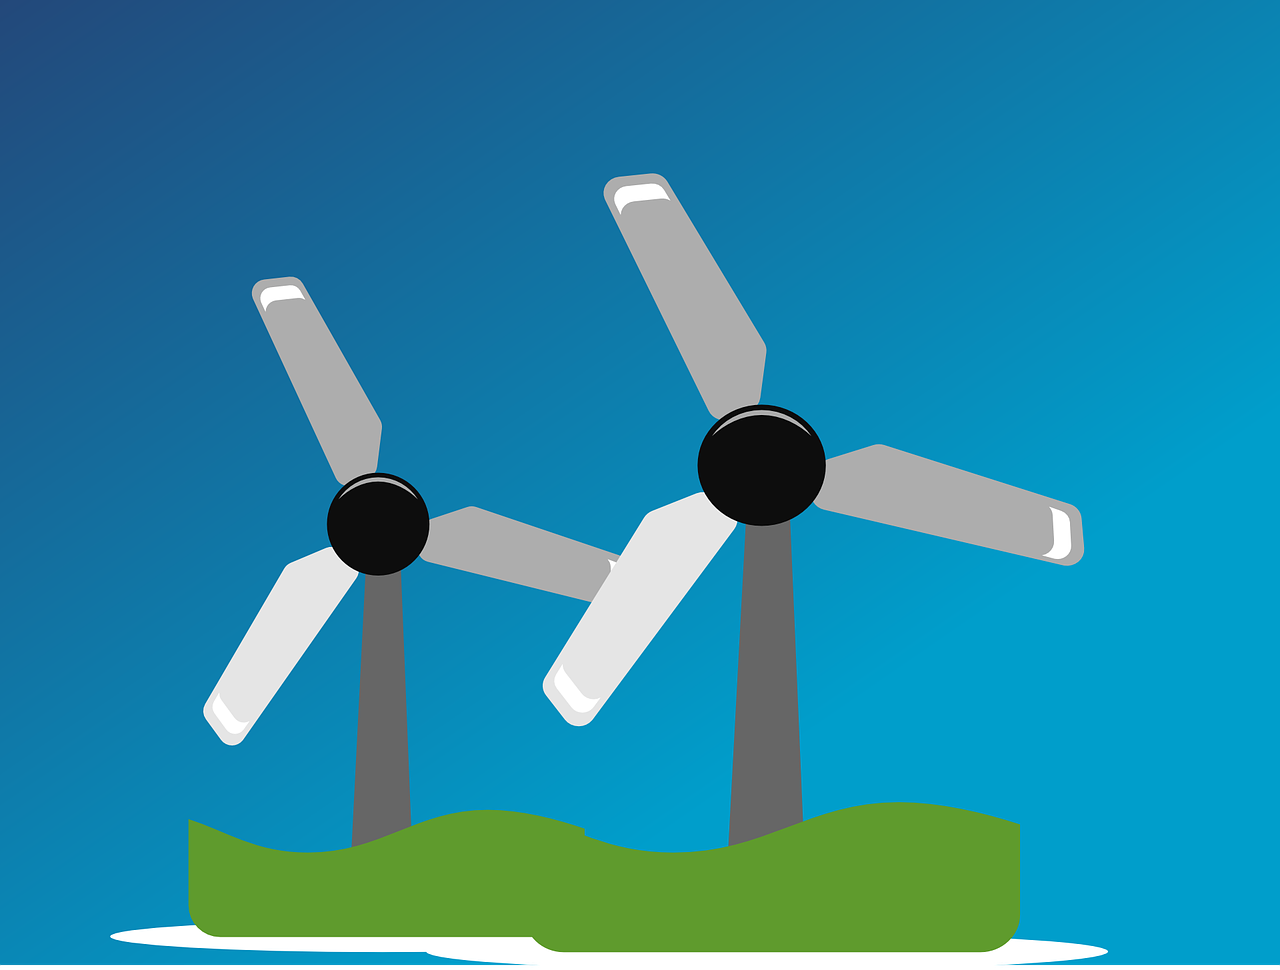
\includegraphics[width=2\textwidth]{img/enrgy.png}}; \\
\node[defaultStyle, draw, onslide={<3->{highlight2}}](s4){
\includegraphics[width=\textwidth]{img/woman2.png}};      \& \\
};

\draw[onslide={<2->{highlight}}] (s1) -- (c1);
\draw[] (s1) -- (c2);

\draw[onslide={<2->{highlight}}] (s2) -- (c1);
\draw[] (s2) -- (c3);

\draw[onslide={<2->{highlight}}] (s3) -- (c2);

\draw[onslide={<2->{highlight}}] (s4) -- (c3);
\draw[] (s4) -- (c2);
%
%\draw[onslide={<1-2>{highlight}}] (z) -- (3);
%\draw[onslide={<3>{highlight}}] (z) -- (2);
%
%\draw[onslide={<1-2>{highlight}}] (t) -- (2);
%\draw[] (t) -- (1);
%\draw[onslide={<3>{highlight}}] (t) -- (5);
%\draw[] (t) -- (3);
%\draw[] (t) -- (4);
%\draw[onslide={<1>{highlight}}] (u) -- (4);
%\draw[] (u) -- (3);
%\draw[] (u) -- (5);
%\draw[] (u) -- (6);
\end{tikzpicture}
\end{center}
\onslide<2->{This \alert{assignment} respects students' preferences (edges) \onslide<3->{but ignores {\color{CornflowerBlue} companies' preferences}.}}
%\onslide<4->{\tiny OK, es ist nicht wirklich ein \emph{Matching} da Firmen mehr als einen Studenten betreuen \ldots }
\end{frame}

\begin{frame}[fragile]{Mentor Matching: Constraint Model}
\begin{lstlisting}
int: n; set of int: STUDENT = 1..n;
int: m; set of int: COMPANY = 1..m;

% assign students to companies
array[STUDENT] of var COMPANY: worksAt;


int: minPerCompany = 1; int: maxPerCompany = 3;
constraint global_cardinality_low_up ( 
           worksAt, [c | c in COMPANY], 
           [minPerCompany | c in COMPANY], 
           [maxPerCompany | c in COMPANY]); 
           
solve 
search pvs_BAB();
\end{lstlisting}
\end{frame}

\begin{frame}[fragile]{Mentor Matching: FAS* Instance}
\begin{lstlisting}
% fas2016.mzn

n = 5; % students
m = 3; % companies

% student names for better readability 
int: britney = 1;
int: christina = 2;
int: drdre = 3; 
int: eminem = 4; 
int: falco = 5; 

% company names 
int: disney = 1;
int: warner = 2;
int: uniaugsburg = 3;
\end{lstlisting}

\end{frame}

\begin{frame}[fragile]{Mentor Matching: Preferences}
\begin{lstlisting}
PVS: students = new ConstraintRelationships("students") {
   soft-constraint britneyDisney : 'worksAt[britney] = disney';
   soft-constraint britneyWarner : 'worksAt[britney] = warner';
   soft-constraint eminemUnia : 'worksAt[eminem] = uniaugsburg';
   crEdges : '[|  mbr.britneyDisney , mbr.britneyWarner | mbr.eminemUnia, mbr.britneyDisney |]';
   useSPD: 'true' ;
}; 

PVS: companies = new ConstraintRelationships("companies") {
   soft-constraint disneyChristina : 'worksAt[christina] = disney';
   soft-constraint disneyFalco : 'worksAt[falco] = disney';
   soft-constraint uniaugsburg : 'worksAt[britney] = uniaugsburg';
   
   crEdges : '[| mbr.disneyFalco, mbr.uniaugsburg |]';
   useSPD: 'true' ;
}; 
\end{lstlisting}
\end{frame}

\begin{frame}[fragile]{Mentor Matching: Behavior I}
\begin{lstlisting}
solve ToWeighted(students) lex ToWeighted(companies);
\end{lstlisting}
\begin{Verbatim}[fontsize=\small]
Intermediate solution:worksAt = [3, 2, 1, 1, 1]
Valuations: penCompanies = 1; penStudents = 6
----------
Intermediate solution:worksAt = [2, 3, 1, 1, 1]
Valuations: penCompanies = 3; penStudents = 3
----------
Intermediate solution:worksAt = [1, 1, 2, 3, 1]
Valuations: penCompanies = 2; penStudents = 3
----------
Intermediate solution:worksAt = [2, 1, 1, 3, 1]
Valuations: penCompanies = 2; penStudents = 2
----------
==========
\end{Verbatim}

\end{frame}

\begin{frame}[fragile]{Mentor Matching: Behavior II}
\begin{lstlisting}
solve ToWeighted(companies) lex ToWeighted(students);
\end{lstlisting}
\begin{Verbatim}[fontsize=\small]
Intermediate solution:worksAt = [3, 2, 1, 1, 1]
Valuations: penCompanies = 1; penStudents = 6
----------
Intermediate solution:worksAt = [3, 1, 2, 1, 1]
Valuations: penCompanies = 0; penStudents = 6
----------
Intermediate solution:worksAt = [3, 1, 2, 3, 1]
Valuations: penCompanies = 0; penStudents = 5
----------
==========
\end{Verbatim}

\end{frame}


\begin{frame}[fragile]{Mentor Matching: Winter Term 15/16}
\begin{itemize}
\item Collected preferences from emails 

\begin{parchment}
\begin{verbatim}
"the favorites":
1. JuneDied-Lynx- HumanIT
2. Cupgainini
 
"I could live with that":
3. Seamless-German
4. gsm systems
5. Yiehlke
 
"I think, we won't be happy":
6. APS
7. Delphi Databases
\end{verbatim} 
\end{parchment}
\end{itemize}
\end{frame}

\begin{frame}[fragile]{Mentor Matching: Winter Term 15/16}
\begin{itemize}
\item Priority for \alert{students}
\begin{itemize}
\item[-] What are companies supposed to do with unhappy students?
\end{itemize}
\item Search space: 7 Companies for 16 students $\rightarrow 7^{16} = 3.3233 \cdot 10^{13}$
\vspace*{2ex}
\item Led to a constraint problem with
\begin{itemize}
\item[-] 77 students' preferences (soft constraints) of 16 students
\item[-] in total 114 soft constraints (37 company preferences) 
\end{itemize}

\vspace*{2ex}

\item \emph{Proven} optimal solution
\begin{itemize}
\item[-] 6 minutes 
\end{itemize}
\end{itemize}
\end{frame}


%
\begin{frame}{Evaluation}
\begin{itemize}
\item Direkter Vergleich schwierig
\item Kein anderes System implementiert PVS (oder c-Semiringe)
\item $\rightarrow$ Dafür unterstützt \texttt{toulbar2} Weighted CSP und \emph{Cost Function Networks}
\item[] (der einzig frei verfügbare \emph{Soft-Constraint-Solver})
\end{itemize}

\vspace*{2ex} \pause 

\begin{itemize}
\item Daher Beschränkung auf \emph{Weighted CSP} für die Evaluierung
\item Abbildung aus Constraint-Relationships
\item Probleme sind Variationen von 5 Problemen aus den MiniZinc-Benchmarks\footnote{\url{https://github.com/MiniZinc/minizinc-benchmarks}} (erweitert um Soft Constraints in PVS)
\end{itemize}


\end{frame}

\begin{frame}{Rahmenbedingungen}
\begin{itemize}
\item Eingesetzte Solver
\begin{itemize}
\item[-] JaCoP
\item[-] Gecode
\item[-] Google OR-Tools
\item[-] G12
\item[-] Choco
\item[-] \texttt{toulbar2}
\end{itemize}

\vspace*{2ex}

\item Eingesetzte Probleme (insgesamt 15 Instanzen)
\begin{itemize}
\item[-] Soft-Queens
\item[-] Photo-Platzierung
\item[-] Talent-Scheduling
\item[-] On-Call-Rostering
\item[-] Multi-Skilled Project Scheduling Problem
\end{itemize}

\vspace*{2ex}
\item Timeout: 10 Minuten
\end{itemize}
\end{frame}

\begin{frame}{Resultate: Kleine Probleme} \small
\textbf{Photo-Platzierung und Soft-Queens} 

\begin{table}[t]
%\vspace*{1.3ex}% Fill page
\caption{\normalfont Werte in Klammern geben die beste gefundene Lösung nach Timeout an; Da Weighted CSP $\rightarrow$ Minimierung. Zeiten in Sekunden.}
%
%\newcolumntype{C}{>{\centering\arraybackslash}X}
\begin{tabularx}{\columnwidth}{lcccccc}
  \toprule
  & OR-Tools & Gecode & Choco & JaCoP & G12 & \texttt{toulbar2} \\
  \midrule 
  Photo \\
  \midrule
  photo1 & \textbf{0.18} & 0.19 & 0.41 & 0.54 & 3.38 & \hFirst{0.4}\\
  photo2 & 1.06 & 2.98 & \textbf{0.52} & 2.92 & 35.3 & \hFirst{0.55} \\
  \midrule 
  Soft-Queens \\
  \midrule 
  $n = 8$ & \textbf{0.03} & 0.03 & 0.46 & 0.18 & 0.03 & \hFirst{0.27} \\
  $n = 16$ & \textbf{0.03} & 0.04 & 0.5 & 0.22 & 0.05 & \hFirst{0.28} \\ 
  $n = 30$ & \textbf{0.04} (0) & 600 (4) & 0.55 (0) & 187.86 (0) & 600 (4)  & \hFirst{0.58 (0)} \\ 
  \bottomrule                             
\end{tabularx}
\label{tab:closing}
\end{table}

\end{frame}

\begin{frame}{Resultate: Mittlere Probleme} \small
\textbf{Talent-Scheduling und On-Call Rostering} 

\begin{table}[t]
%\vspace*{1.3ex}% Fill page
\caption{\normalfont Werte in Klammern geben die beste gefundene Lösung nach Timeout an; Da Weighted CSP $\rightarrow$ Minimierung. Zeiten in Sekunden.}
%
%\newcolumntype{C}{>{\centering\arraybackslash}X}
\begin{tabularx}{\columnwidth}{lcccccc}
  \toprule
  & OR-Tools & Gecode & Choco & JaCoP & G12 & \texttt{toulbar2} \\
  \midrule 
  Talents \\
  \midrule
  small & \textbf{0.03} & 0.03 & 0.35 & 0.16 & 0.04 & \hFirst{2.28}\\
  concert & \textbf{0.05} & 0.05 & 0.47 & 0.24 & 0.07 & \hFirst{16.98} \\
  film103 & \textbf{2.23} & 67.69 & 7.48 & 3.01 & 9.3 & -- \\
  \midrule 
  Rostering \\
  \midrule 
  4s-10d\footnote{s bezeichnet ``staff'', d ``days''} & \textbf{0.14} & 0.17 & 1.53 & 0.64 & 0.22 & \hFirst{0.81} \\
  4s-23d & \textbf{2.59} & 2.92 & 5.68 & 4.06 & 4.49 & \hFirst{3.98} \\ 
  10s-50d & 600 (6) & 600 (6) & 600 (14) & 600 (10) & 600 (10) & \hFirst{\textbf{87.18} (1)} \\ 
  \bottomrule                             
\end{tabularx}
\label{tab:closing}
\end{table}

\end{frame}


\begin{frame}{Resultate: Große Probleme} \small
\textbf{Multi-Skilled Project Scheduling Problem} 

\begin{table}[t]
%\vspace*{1.3ex}% Fill page
\caption{\normalfont Werte in Klammern geben die beste gefundene Lösung nach Timeout an; Da Weighted CSP $\rightarrow$ Minimierung. Zeiten in Sekunden.}
%
%\newcolumntype{C}{>{\centering\arraybackslash}X}
\begin{tabularx}{\columnwidth}{lcccccc}
  \toprule
  & OR-Tools & Gecode & Choco & JaCoP & G12 & \texttt{toulbar2} \\
  \midrule 
  MSPSP \\
  \midrule
  easy\_01 & \textbf{0.2} & 0.32 & 1.26 & 0.94 & 0.27 & --\\
  medium\_01 & \textbf{0.19} & 0.22 & 1.35 & 0.67 & 0.21 & --\\
  hard\_02 & 0.37 & \textbf{0.33} & 1.59 & 1.01 & 0.37 & 600 (--)\\
  hard\_04 & 0.27 & \textbf{0.25} & 1.62 & 0.86 & 0.28 & --\\
     \bottomrule                             
\end{tabularx}
\label{tab:closing}
\end{table}

\end{frame}

%
\begin{frame}{Kooperationen}
\begin{itemize}
\item[] \alert{Konzepte, Sprachdesign MiniBrass}
\begin{itemize}
\item[-] AS, Alexander Knapp, Gerrit Anders, Oliver Kosak
\end{itemize}
\item[] \alert{Anwendungen, Multiagenten-Einsatz}
\begin{itemize}
\item[-] Alexander Schubert (MSc-Thesis: Einsatz von Voting-Verfahren), Markus Tolls (MSc-Thesis: Formalisierung von Task-Allocation-Problemen)
\end{itemize}
\end{itemize}
\end{frame}

\begin{frame}{Outreach}
\begin{itemize}
\item Vortrag Helmholtz-Zentrum München
\item Vortrag FH Hagenberg
\item Tutorial @ SASO 2016
\end{itemize}
\end{frame}


%

\begin{frame}[allowframebreaks]
        \frametitle{References}
        \bibliographystyle{apalike}
        \bibliography{references}
\end{frame}


\end{document}

